% !TEX encoding = utf8
% ============================================================================
%  Design and Development of an Offline-First Mobile Application
%  for Field Data Collection -- Master's Thesis
%
%  Built on the official Politecnico di Torino `toptesi` thesis class
%  (https://www.overleaf.com/latex/templates/politecnico-di-torino-thesis-template/cmpmxftwvvbr).
%  Compiles on Overleaf (pdfLaTeX) and on a TeX Live install that has the
%  `toptesi` package. See README.md for the full compile recipe.
% ============================================================================

% One-sided master's thesis. For double-sided printing use instead:
% \documentclass[b5paper,12pt,twoside,cucitura,tipotesi=magistrale,stile=classica]{toptesi}
\documentclass[a4paper,12pt,cucitura,tipotesi=magistrale,stile=classica]{toptesi}

% ---------- Encoding / fonts ----------
\usepackage[utf8]{inputenc}
\usepackage[T1]{fontenc}
\usepackage{lmodern}
\usepackage{csquotes}

% ---------- Maths ----------
\usepackage{amsmath}
\usepackage{amssymb}

% ---------- Graphics / diagrams ----------
\usepackage{graphicx}
\usepackage[export]{adjustbox}
\usepackage{xcolor}
\usepackage{tikz}
\usetikzlibrary{shapes.geometric,arrows.meta,positioning,fit,backgrounds,calc,decorations.pathreplacing}
\usepackage{pgfplots}
\pgfplotsset{compat=1.18}
\usepackage{subcaption}
\usepackage{float}

% ---------- Tables ----------
\usepackage{booktabs}
\usepackage{longtable}
\usepackage{multirow}
\usepackage{tabularx}
\newcolumntype{L}{>{\raggedright\arraybackslash}X}

% ---------- Lists ----------
\usepackage{enumitem}

% ---------- Code listings ----------
\usepackage{listings}
\definecolor{codebg}{RGB}{245,245,245}
\definecolor{codekeyword}{RGB}{0,90,150}
\definecolor{codecomment}{RGB}{110,110,110}
\definecolor{codestring}{RGB}{140,20,20}
\lstdefinelanguage{Kotlin}{
  keywords={package, import, class, interface, object, fun, val, var, return, if, else, for, while, when, is, in, out, this, super, null, true, false, override, private, public, protected, internal, companion, data, enum, sealed, suspend, try, catch, finally, throw, as, typealias, expect, actual, by, lazy, init, constructor},
  keywordstyle=\color{codekeyword}\bfseries,
  sensitive=true,
  comment=[l]{//},
  morecomment=[s]{/*}{*/},
  commentstyle=\color{codecomment}\itshape,
  string=[b]",
  stringstyle=\color{codestring},
  morestring=[b]',
}
\lstset{
  backgroundcolor=\color{codebg},
  basicstyle=\ttfamily\footnotesize,
  breaklines=true,
  breakatwhitespace=false,
  frame=single,
  rulecolor=\color{black!20},
  numbers=left,
  numberstyle=\tiny\color{black!50},
  numbersep=8pt,
  tabsize=2,
  showstringspaces=false,
  captionpos=b,
  xleftmargin=1.5em,
}

% ---------- Glossary / acronyms ----------
\usepackage[nogroupskip,toc]{glossaries}
\makeglossaries
% ============================================================================
%  Glossary and acronym definitions (glossaries package).
%  Printed by \printglossary in thesis.tex. Referenced in text with
%  \gls{...} / \acrshort{...} / \acrfull{...} if desired.
% ============================================================================

% ---- Acronyms --------------------------------------------------------------
\newacronym{kmp}{KMP}{Kotlin Multiplatform}
\newacronym{mvvm}{MVVM}{Model--View--ViewModel}
\newacronym{dao}{DAO}{Data Access Object}
\newacronym{lww}{LWW}{Last-Write-Wins}
\newacronym{crdt}{CRDT}{Conflict-free Replicated Data Type}
\newacronym{crud}{CRUD}{Create, Read, Update, Delete}
\newacronym{baas}{BaaS}{Backend-as-a-Service}
\newacronym{sus}{SUS}{System Usability Scale}
\newacronym{uuid}{UUID}{Universally Unique Identifier}
\newacronym{ui}{UI}{User Interface}
\newacronym{ksp}{KSP}{Kotlin Symbol Processing}
\newacronym{fr}{FR}{Functional Requirement}
\newacronym{nfr}{NFR}{Non-Functional Requirement}
\newacronym{ofr}{OFR}{Offline-specific Requirement}

% ---- Glossary terms --------------------------------------------------------
\newglossaryentry{offlinefirst}{
  name={offline-first},
  description={A design approach in which the local device is the primary
  source of truth for user data and the network is an optional,
  asynchronous synchronization channel, so the application is fully usable
  with no connectivity}
}

\newglossaryentry{lastwritewins}{
  name={last-write-wins},
  description={A conflict-resolution policy that, when two versions of a
  record diverge, keeps the version with the more recent modification
  timestamp and discards the other}
}

\newglossaryentry{syncstatus}{
  name={sync status},
  description={A per-record field indicating the relationship between the
  local copy of the record and the backend: pending, synced, failed, or
  deleted-pending}
}

\newglossaryentry{idempotent}{
  name={idempotent},
  description={A property of an operation whereby applying it multiple times
  produces the same result as applying it once; here, re-running a
  synchronization must not create duplicate remote records}
}


% ---------- Hyperlinks (load late) + cross-references ----------
\usepackage{hyperref}
\hypersetup{
  pdfpagemode={UseOutlines},
  bookmarksopen,
  pdfstartview={FitH},
  colorlinks=true,
  linkcolor=black,
  citecolor=black,
  urlcolor=blue
}
\usepackage[capitalise,noabbrev]{cleveref}
\crefname{lstlisting}{Listing}{Listings}
\Crefname{lstlisting}{Listing}{Listings}

\setcounter{tocdepth}{3}
\setcounter{secnumdepth}{3}

\begin{document}

% ---------- Front-page metadata & title page ----------
% ============================================================================
%  Front-page metadata for the toptesi \frontespizio command.
%  These are the standard PoliTo toptesi frontpage macros. Edit the bracketed
%  values before submission.
% ============================================================================

\english   % Title page and headings in English. Comment out for Italian.

\ateneo{Politecnico di Torino}
%\nomeateneo{Sede Centrale}

\titolo{Design and Development of an Offline-First Mobile Application for Field Data Collection}
%\sottotitolo{The CampusFix maintenance-reporting case study}

\corsodilaurea{Computer Engineering}

\candidato{Masoud \textsc{Karimi}}

\relatore{Prof.\ [Supervisor Name]}
%\secondorelatore{Prof.\ [Co-supervisor Name]}
%\tutoreaziendale{Dr.\ [Company Tutor]}

% \sedutadilaurea may be called twice: academic year, then session month.
\sedutadilaurea{\textsc{Academic~year} 2025-2026}
\sedutadilaurea{\textsc{[Defense Month]} 2026}

% The official PoliTo logo. The Overleaf PoliTo template ships a `logopolito`
% image; add that file to the project and uncomment the next line to show it.
% Without it, \frontespizio still produces a valid (logo-less) title page.
%\logosede{logopolito}

% ---- English strings for the title page (toptesi conditional block) --------
\iflanguage{english}{%
  \CorsoDiLaureaIn{Master of Science in\space}
  \TesiDiLaurea{Master's Thesis}
  \InName{in}
  \CandidateName{Candidate}
  \AdvisorName{Supervisor}
  \TutorName{Tutor}
  \NomeTutoreAziendale{Company Tutor}
  \NomePrimoTomo{First volume}
  \NomeSecondoTomo{Second Volume}
  \NomeTerzoTomo{Third Volume}
  \NomeQuartoTomo{Fourth Volume}
}{}

\frontespizio

% ---------- FRONT MATTER (roman page numbers) ----------
\frontmatter
\pagenumbering{roman}

% -- Dedication (optional; personalize or remove) --
\vspace*{\stretch{1}}
\begin{flushright}
  \noindent\textit{[Optional dedication.]}
\end{flushright}
\vspace*{\stretch{6}}
\cleardoublepage

% -- Abstract --
\sommario
% Body only: the heading is supplied by toptesi's \sommario in thesis.tex.

Mobile applications used in the field -- on construction sites, in
agriculture, during humanitarian response, or, as in the scenario studied
in this thesis, for facility maintenance reporting on a university campus
-- routinely operate in environments where network connectivity is
intermittent, slow, or entirely absent. Applications that assume an
always-on connection degrade badly in these conditions: user input is
lost, screens hang waiting for a server response, and users lose trust in
the tool. \emph{Offline-first} design addresses this by treating the local
device as the primary source of truth and the network as an optional,
asynchronous channel for synchronization.

This thesis presents the design, implementation, and evaluation of
\emph{CampusFix}, an offline-first mobile application for reporting
maintenance problems (broken projectors, damaged furniture, Wi-Fi outages,
HVAC issues, missing lab equipment) on a university campus. The application
is built with Kotlin Multiplatform and Compose Multiplatform, sharing a
single codebase across Android and iOS, and persists data locally in an
embedded SQLite database accessed through the Room persistence library. A
dedicated synchronization module observes device connectivity, queues
locally-created reports, and pushes them to a Firebase Firestore backend
when a connection becomes available, exposing an explicit per-report sync
status (\texttt{pending}, \texttt{synced}, \texttt{failed},
\texttt{deleted\_pending}) so that users always know whether their data has
left the device.

The thesis makes three contributions. First, it distills the engineering
questions that recur when building offline-first mobile software -- what to
store locally, when to trigger synchronization, how to surface sync state
to the user, and how to resolve conflicting edits -- into a concrete
requirements analysis grounded in a realistic scenario. Second, it presents
a layered system architecture (presentation, domain, data, and
synchronization layers) and a synchronization algorithm based on a
local-first write path with a background push-and-reconcile strategy,
together with a last-write-wins conflict resolution policy suitable for
low-contention, single-owner records such as maintenance reports. Third, it
evaluates the resulting system against six scenarios -- offline creation,
delayed synchronization, failed synchronization, large sync queues,
concurrent edit conflicts, and end-user usability -- discussing both the
quantitative behaviour of the synchronization module and the qualitative
experience of first-time users.

The results indicate that a relatively small, well-isolated synchronization
module is sufficient to make a CRUD-style field-reporting application fully
usable offline, that connectivity-triggered background sync keeps the
perceived latency of ``going back online'' low, and that a strict
last-write-wins policy is an acceptable trade-off for this class of
application, provided the user interface makes the sync status visible at
all times. The thesis closes with a discussion of the current
implementation's limitations -- most notably that synchronization is
presently a one-directional push from device to server rather than a full
bidirectional merge -- and outlines the engineering work required to close
that gap.


% -- Acknowledgements --
\ringraziamenti
% Body only: the heading is supplied by toptesi's \ringraziamenti in thesis.tex.

[This page is a placeholder -- personalize it before submission.]

I would like to thank my supervisor, Prof.\ [Supervisor Name], for the
guidance, critical questions, and patience throughout the development of
this thesis.

I would like to thank the five volunteers who took part in the usability
test described in Chapter~\ref{ch:evaluation} for their time and honest
feedback.

Finally, I thank my family and friends for their continuous support during
this degree.


% -- Table of contents, list of figures, list of tables --
\tablespagetrue\figurespagetrue
\indici

% ---------- MAIN MATTER (arabic page numbers) ----------
\mainmatter
\pagenumbering{arabic}

\chapter{Introduction}
\label{ch:introduction}

\section{Motivation}
\label{sec:motivation}

Mobile software is increasingly assumed to be "always connected." Modern
frameworks, backend-as-a-service platforms, and UI toolkits are built around
the request/response cycle: an action in the interface triggers a network
call, and the interface waits for -- or reacts to -- the server's answer.
This assumption is reasonable for a large class of consumer applications
used indoors, in urban areas, on stable Wi-Fi or 4G/5G connections. It is a
poor assumption for the growing class of applications used \emph{in the
field}: on construction sites, in warehouses and basements, in rural areas,
during disaster response, in agriculture, and -- the scenario adopted in
this thesis -- by facility-maintenance staff and building occupants moving
through a large university campus.

In all of these environments, connectivity is not binary. It is
intermittent (available in some rooms, absent in others), variable in
quality (a slow, high-latency link that behaves worse than no link at all
for a synchronous request), and sometimes simply unavailable for extended
periods (elevators, basements, remote buildings, network outages). An
application that treats the network as always present will, in these
conditions, either block the user interface while waiting for a server that
cannot be reached, silently drop user input, or crash outright. None of
these outcomes are acceptable for an application whose entire purpose is to
let a user \emph{capture something at the moment it happens} -- a broken
projector noticed while walking past a lecture hall, a damaged chair found
during a room inspection -- because if the app does not let the user record
the observation there and then, the observation is very often never
recorded at all.

\emph{Offline-first} is the name given to a family of design and
engineering practices that respond to this reality by inverting the default
assumption: the local device, not the remote server, is treated as the
primary source of truth for user-generated data, and the network is treated
as an optional, asynchronous channel used to propagate that data to a
backend and to other devices. An offline-first application is, by
definition, fully usable with no network connection; when connectivity is
available, a synchronization process reconciles local and remote state in
the background, ideally without the user having to do anything beyond being
informed of the outcome.

Building an offline-first application well is a genuinely different
engineering problem from building a "normal" client-server application with
some caching bolted on. It requires an explicit local persistence model,
an explicit representation of "this record has not yet reached the
server," an explicit strategy for deciding \emph{when} to attempt
synchronization, and an explicit -- even if intentionally simple --
strategy for what happens when the same record has been modified in two
places before either side has seen the other's change. Consumer
applications like Google Docs, Notion, or messaging apps solve versions of
this problem with considerable engineering investment (operational
transformation, CRDTs, vector clocks). The central question this thesis
asks is more modest and more practical: \emph{what is the smallest,
most maintainable offline-first architecture that is sufficient for a
CRUD-style field-reporting application}, and what engineering trade-offs
does that architecture force the developer to make explicit?

\section{Offline-First Applications}
\label{sec:offline-first-background}

The term "offline first" was popularized in mobile and web development
around 2013--2014 as a reaction to the "mobile first, then make it work
offline" pattern, which tends to produce applications where offline support
is a thin, unreliable layer retrofitted onto a fundamentally online
architecture~\cite{offlinefirst2013}. The offline-first position instead
argues that offline behaviour should be a first-class design constraint
from the start of a project, because retrofitting it later requires
touching almost every part of the data layer.

At the core of offline-first engineering is a shift in where reads and
writes are directed. \Cref{fig:online-vs-offline} contrasts the two
architectures at a high level. In a conventional "online-only" design
(\cref{fig:online-vs-offline}, left), the UI issues a request directly to
the backend and the operation's success or failure is determined
synchronously by the network round trip. In an offline-first design
(\cref{fig:online-vs-offline}, right), the UI only ever talks to the local
data store; a separate synchronization component is responsible for
propagating local changes to the backend when a network path exists, and
for pulling remote changes back down. The user-visible effect of a create,
update, or delete operation is therefore always fast and always available,
because it depends only on local disk I/O, never on the network.

\begin{figure}[htbp]
  \centering
  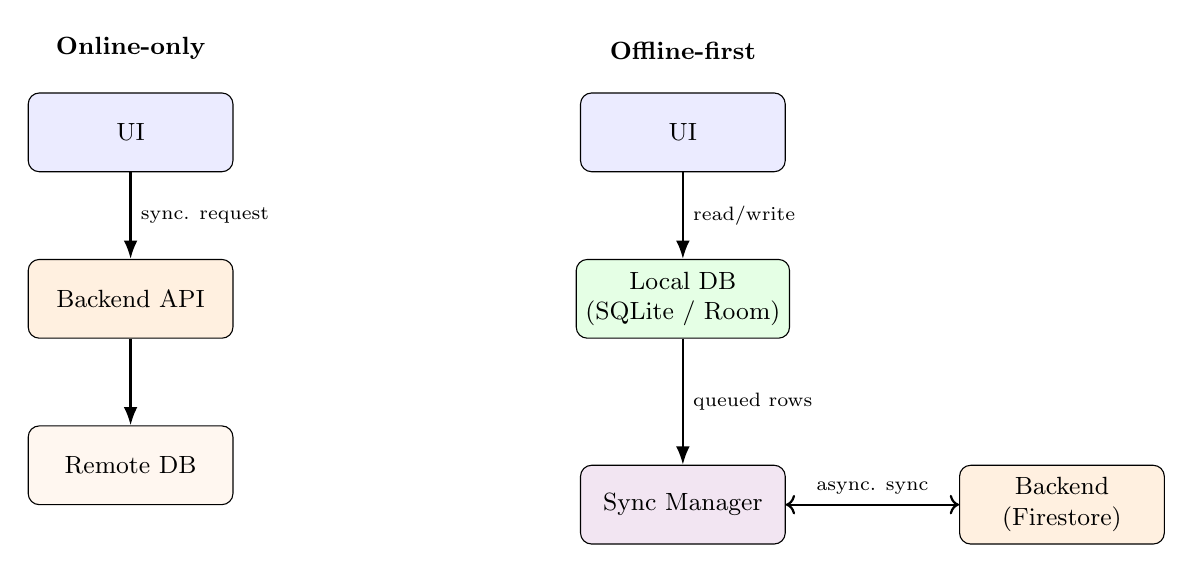
\begin{tikzpicture}[
      node distance=1.1cm and 1.6cm,
      box/.style={draw, rounded corners, minimum width=2.6cm, minimum height=1cm, align=center, font=\small},
      arrow/.style={-Latex, thick}
    ]
    % Online-only
    \node[box, fill=blue!8] (ui1) {UI};
    \node[box, fill=orange!12, below=of ui1] (backend1) {Backend API};
    \node[box, fill=orange!6, below=of backend1] (db1) {Remote DB};
    \draw[arrow] (ui1) -- node[right, font=\scriptsize]{sync. request} (backend1);
    \draw[arrow] (backend1) -- (db1);
    \node[font=\small\bfseries, above=0.3cm of ui1] {Online-only};

    % Offline-first
    \node[box, fill=blue!8, right=4.4cm of ui1] (ui2) {UI};
    \node[box, fill=green!10, below=of ui2] (local2) {Local DB\\ (SQLite / Room)};
    \node[box, fill=violet!10, below=1.6cm of local2] (sync2) {Sync Manager};
    \node[box, fill=orange!12, right=2.2cm of sync2] (backend2) {Backend\\ (Firestore)};
    \draw[arrow] (ui2) -- node[right, font=\scriptsize]{read/write} (local2);
    \draw[arrow] (local2) -- node[right, font=\scriptsize]{queued rows} (sync2);
    \draw[arrow, <->] (sync2) -- node[above, font=\scriptsize]{async. sync} (backend2);
    \node[font=\small\bfseries, above=0.3cm of ui2] {Offline-first};
  \end{tikzpicture}
  \caption{Data flow in an online-only architecture versus an offline-first
  architecture. In the offline-first case the UI never blocks on the
  network: every read and write is served by the local database, and
  synchronization runs as an independent, asynchronous process.}
  \label{fig:online-vs-offline}
\end{figure}

This shift has consequences that ripple through the whole stack:

\begin{itemize}
  \item \textbf{Local persistence becomes a primary concern, not a cache.}
  The local database must be able to represent every state a record can be
  in, including states that have no meaning on the server (e.g. "created
  locally, not yet uploaded").
  \item \textbf{Identity must be decided before the server is involved.}
  If a report is created offline, it needs an identifier the moment it is
  created, before any server-assigned identifier exists. This typically
  means client-generated identifiers (UUIDs) coexisting with
  server-assigned identifiers.
  \item \textbf{Synchronization is a background process, not a request
  handler.} It must be triggered by connectivity changes and/or periodic
  timers, must be resumable after being interrupted, and must be
  idempotent -- running it twice must not create duplicate data.
  \item \textbf{Conflicts become possible, and must be resolved by policy,
  not by accident.} Two devices -- or a device and a server-side edit --
  can modify the same record while disconnected from each other. The
  application must define, even if only in the simplest possible way, what
  happens when those two versions are reconciled.
  \item \textbf{The user needs visibility into synchronization state.}
  Because writes are decoupled from network availability, the UI must
  communicate whether a given piece of data is safely stored on the server
  or still only local, or the offline-first property becomes a source of
  anxiety rather than resilience.
\end{itemize}

These five concerns map directly onto the "Research/engineering questions"
that motivate this thesis (\cref{sec:objectives}), and onto the chapters
that follow: \cref{ch:requirements} turns them into concrete requirements,
\cref{ch:design} turns the requirements into an architecture, and
\cref{ch:implementation} shows how that architecture is realised in code.

\section{Field Data Collection as a Case Study}
\label{sec:case-study}

Field data collection is a natural and well-studied application area for
offline-first design~\cite{brunette2013odk,hartung2010open}. It shares the
same shape across many domains -- agriculture, epidemiology, environmental
monitoring, humanitarian logistics, facility maintenance -- namely, a field
worker observes something, records structured data about it (often with a
photo and a location), and that data needs to eventually reach a central
system where it can be aggregated, triaged, and acted upon. The
observation happens where it happens; the network may or may not be
available at that exact place and time.

This thesis instantiates the field data collection problem with a scenario
that is small enough to implement and evaluate within the scope of a
master's thesis, yet representative of the harder domains listed above: a
mobile application, referred to throughout this document as
\textbf{CampusFix}, that lets students, faculty, and staff of a university
campus report facility problems as they encounter them. Representative
report categories include:

\begin{itemize}
  \item a broken or missing projector in a lecture hall;
  \item a damaged chair or desk;
  \item a Wi-Fi outage or coverage problem in a specific building/room;
  \item an air-conditioning or heating malfunction;
  \item missing or malfunctioning laboratory equipment.
\end{itemize}

A user of CampusFix is frequently \emph{exactly} in the situation
offline-first design targets: standing in a basement lab with no signal,
noticing a broken piece of equipment, and wanting to log it before moving
on and forgetting the details. If the application requires a live
connection to save that report, the report is lost, or the user is forced
to remember to re-open the app later -- which, in practice, means the
report is usually never filed. CampusFix must therefore let the user
complete the entire "create a report" flow with zero network availability,
and must reliably deliver that report to the facilities-management backend
once the device regains connectivity, without requiring the user to
remember to do anything.

\section{Problem Statement}
\label{sec:problem-statement}

Given the scenario above, this thesis addresses the following problem:
\emph{design, implement, and evaluate a mobile application that lets a user
create, view, and manage field reports with full functionality while
offline, that synchronizes those reports with a backend transparently and
reliably once connectivity returns, that communicates synchronization state
to the user at all times, and that resolves the simple conflicts that can
arise when a report is modified both locally and on the server}, using a
technology stack -- Kotlin Multiplatform for the client, SQLite/Room for
local storage, and Firebase (Firestore and Authentication) for the backend
-- that is realistic for a small engineering team to adopt and maintain.

\section{Objectives and Contributions}
\label{sec:objectives}

The thesis pursues the following concrete objectives, mirroring the
engineering questions posed in the project brief:

\begin{enumerate}[label=\textbf{O\arabic*.}]
  \item \textbf{Usability without connectivity.} Determine what UI/UX and
  architectural patterns keep a mobile app fully usable when internet
  connectivity is absent, and implement them for the report creation,
  listing, and detail flows.
  \item \textbf{Local data model.} Determine what data must be stored
  locally (and in what form) so that the application never depends on a
  network round trip for a core operation, and design a local schema that
  supports this.
  \item \textbf{Synchronization triggers.} Determine when and how
  synchronization should be triggered -- on connectivity change, on app
  start, periodically, or manually -- and implement a connectivity-aware
  synchronization module.
  \item \textbf{Sync-state visibility.} Determine how to communicate
  upload state to the user (pending / synced / failed) so that offline
  operation is legible rather than opaque.
  \item \textbf{Conflict resolution.} Determine what conflict-resolution
  strategy is acceptable for this class of application, and implement the
  simplest strategy that meets that bar.
\end{enumerate}

Correspondingly, the thesis contributes:

\begin{enumerate}[label=\textbf{C\arabic*.}]
  \item A requirements analysis (\cref{ch:requirements}) that separates
  functional requirements from the offline-specific non-functional
  requirements that are often left implicit in mobile app specifications.
  \item A layered system architecture and synchronization algorithm
  (\cref{ch:design}) for a Kotlin Multiplatform, Room-backed,
  Firestore-synchronized field-reporting application.
  \item A working implementation (\cref{ch:implementation}) of that
  architecture, shared across Android and iOS from a single Kotlin
  codebase, described down to the level of the actual data access objects,
  synchronization loop, and connectivity observers used.
  \item An evaluation (\cref{ch:evaluation}) of the system's offline
  behaviour, synchronization performance, conflict handling, and usability,
  together with an honest discussion of the current implementation's
  limitations, in particular that synchronization today is a one-directional
  push rather than a full bidirectional merge.
\end{enumerate}

\section{Thesis Structure}
\label{sec:structure}

The remainder of this thesis is organized as follows.
\Cref{ch:requirements} analyzes the functional and non-functional
requirements of CampusFix, with particular attention to the requirements
that are specific to offline operation. \Cref{ch:design} presents the
system architecture: the mobile application's internal layering, the local
database schema, the backend structure, and the design of the
synchronization strategy, including the conflict-resolution policy.
\Cref{ch:implementation} describes the implementation of that design using
Kotlin Multiplatform, Compose Multiplatform, Room, and Firebase, walking
through the local database, the connectivity monitor, the synchronization
module, and the user-facing screens. \Cref{ch:evaluation} evaluates the
resulting system against six scenarios covering offline creation, delayed
and failed synchronization, large sync queues, conflicting edits, and
end-user usability. Finally, \cref{ch:conclusions} summarizes the findings,
discusses the limitations of the current implementation, and outlines
directions for future work.

\chapter{Requirements Analysis}
\label{ch:requirements}

This chapter turns the scenario introduced in \cref{ch:introduction} into a
concrete set of requirements. \Cref{sec:stakeholders} identifies the
stakeholders and actors of the system. \Cref{sec:usecases} presents the
core use cases. \Cref{sec:functional-req} lists the functional
requirements. \Cref{sec:nonfunctional-req} lists the non-functional
requirements, and \cref{sec:offline-req} isolates, as a separate section,
the requirements that are specific to offline operation -- since these are
the requirements that most distinguish CampusFix from a conventional CRUD
application and that drive most of the design decisions in
\cref{ch:design}. \Cref{sec:data-req} specifies the data requirements for a
report record, and \cref{sec:constraints} states the constraints and
assumptions under which the requirements were elicited.

\section{Stakeholders and Actors}
\label{sec:stakeholders}

\begin{table}[htbp]
\centering
\caption{Stakeholders and actors of the CampusFix system.}
\label{tab:stakeholders}
\begin{tabularx}{\textwidth}{@{}l X@{}}
\toprule
\textbf{Actor} & \textbf{Description} \\
\midrule
\textbf{Reporter} & Any authenticated campus user (student, faculty, staff)
who creates, views, and manages maintenance reports through the mobile
app. This is the primary actor and the only actor implemented in the
current system. \\
\textbf{Facilities staff} & Consumer of the reports on the backend side.
Out of scope for the mobile application itself, but constrains the shape
of the data stored in Firestore (\cref{sec:data-req}), since that data must
eventually be actionable by this actor through a separate
dashboard/back-office, which is not part of this thesis. \\
\textbf{Synchronization module} & A non-human actor internal to the
system: the background component that moves data between the local
database and Firestore. Modeled as an actor because it initiates actions
(uploads, retries) independently of direct user input. \\
\textbf{Connectivity monitor} & A non-human actor that observes the
device's network state and notifies the synchronization module of
changes. \\
\bottomrule
\end{tabularx}
\end{table}

\section{Use Case Overview}
\label{sec:usecases}

\Cref{fig:usecase} summarizes the use cases supported by the Reporter
actor; \cref{tab:usecase-detail} details the three use cases most relevant
to the offline-first behaviour of the system.

\begin{figure}[htbp]
  \centering
  \begin{tikzpicture}[
      usecase/.style={draw, ellipse, minimum width=3.4cm, minimum height=1cm, align=center, font=\small},
      actor/.style={font=\small},
      >=Latex
    ]
    % Actor
    \node[actor] (actor) at (0,0) {
      \begin{tikzpicture}
        \draw (0,0.5) circle (0.2);
        \draw (0,0.3) -- (0,-0.4);
        \draw (-0.3,-0.1) -- (0.3,-0.1);
        \draw (0,-0.4) -- (-0.25,-0.9);
        \draw (0,-0.4) -- (0.25,-0.9);
      \end{tikzpicture}\\ Reporter
    };

    \node[usecase] (login) at (4,3.2) {Log in / Sign up};
    \node[usecase] (create) at (4,2.0) {Create report};
    \node[usecase] (view) at (4,0.8) {View reports\\(submitted \& pending)};
    \node[usecase] (retry) at (4,-0.4) {Retry failed sync};
    \node[usecase] (status) at (4,-1.6) {Check sync status};
    \node[usecase] (offline) at (8.4,0.8) {Work offline};

    \draw (actor) -- (login);
    \draw (actor) -- (create);
    \draw (actor) -- (view);
    \draw (actor) -- (retry);
    \draw (actor) -- (status);
    \draw[dashed,->] (create) -- node[above,font=\scriptsize]{\guillemotleft include\guillemotright} (offline);
    \draw[dashed,->] (view) -- node[below,font=\scriptsize]{\guillemotleft include\guillemotright} (offline);
  \end{tikzpicture}
  \caption{Use case diagram for the Reporter actor. "Work offline" is
  included by every core use case: none of them require connectivity to
  complete.}
  \label{fig:usecase}
\end{figure}

\begin{table}[htbp]
\centering
\caption{Detail of the three use cases most specific to offline-first
behaviour.}
\label{tab:usecase-detail}
\small
\begin{tabularx}{\textwidth}{@{}l X@{}}
\toprule
\textbf{Create report} & \textbf{Description} \\
\midrule
Actor & Reporter \\
Precondition & User is logged in (a session may be cached locally; see
\cref{sec:offline-req}). \\
Main flow & User opens "New report," fills in title, category,
description, optionally attaches a photo and a location, and submits. \\
Postcondition & A row exists in the local database with
\texttt{sync\_status = pending}. The report is immediately visible in the
report list, tagged as pending. \\
Offline behaviour & Identical to the online flow; no step in the main flow
requires network access. \\
\midrule
\textbf{View submitted and pending reports} & \textbf{Description} \\
\midrule
Actor & Reporter \\
Main flow & User opens the report list; the app displays all reports
belonging to the user, each annotated with its current sync status. \\
Offline behaviour & The list is read entirely from the local database; it
is always available and always reflects the true local state, including
reports not yet on the server. \\
\midrule
\textbf{Retry failed synchronization} & \textbf{Description} \\
\midrule
Actor & Reporter \\
Precondition & At least one report has \texttt{sync\_status = failed}. \\
Main flow & User triggers a manual sync (e.g. pull-to-refresh or a "retry"
action); the app re-attempts upload of all pending/failed reports. \\
Postcondition & Each report's status is updated to \texttt{synced} or
remains \texttt{failed}, depending on the outcome. \\
\bottomrule
\end{tabularx}
\end{table}

\section{Functional Requirements}
\label{sec:functional-req}

\Cref{tab:functional-req} lists the functional requirements (FR), grouped
by feature area and prioritized using the MoSCoW scale (Must, Should,
Could, Won't -- for this iteration).

\begin{longtable}{@{}p{1.4cm}p{8.6cm}p{1.6cm}@{}}
\caption{Functional requirements.}
\label{tab:functional-req}\\
\toprule
\textbf{ID} & \textbf{Requirement} & \textbf{Priority} \\
\midrule
\endfirsthead
\toprule
\textbf{ID} & \textbf{Requirement} & \textbf{Priority} \\
\midrule
\endhead
FR-1 & The system shall let a user create an account and log in with an
email and password. & Must \\
FR-2 & The system shall let a logged-in user create a report consisting of
a title, a category, a free-text description, an optional photo, a
location (building/room), and an automatically-assigned creation
timestamp. & Must \\
FR-3 & The system shall persist every report locally as soon as it is
created, independent of network state. & Must \\
FR-4 & The system shall let a user view the list of their own reports,
both those already synchronized and those still pending. & Must \\
FR-5 & The system shall let a user open a single report to see its full
detail, including its current synchronization status. & Must \\
FR-6 & The system shall let a user edit a previously created report (own
reports only). & Should \\
FR-7 & The system shall let a user delete a previously created report. &
Should \\
FR-8 & The system shall detect when network connectivity becomes
available and automatically attempt to synchronize pending reports. &
Must \\
FR-9 & The system shall let a user manually trigger synchronization. &
Must \\
FR-10 & The system shall display, for every report, one of the following
synchronization statuses: \texttt{pending}, \texttt{synced},
\texttt{failed}, \texttt{deleted\_pending}. & Must \\
FR-11 & The system shall retry synchronization of \texttt{failed} reports
without requiring the user to re-enter data. & Must \\
FR-12 & The system shall apply a defined conflict-resolution policy
(last-write-wins, \cref{sec:conflict-design}) when a report has been
modified both locally and on the server. & Should \\
FR-13 & The system shall upload photos attached to a report to the
backend's file storage and associate the resulting URL with the report
once online. & Could \\
FR-14 & The system shall support attaching a location either via device
GPS or via manual building/room selection. & Could \\
\bottomrule
\end{longtable}

\section{Non-Functional Requirements}
\label{sec:nonfunctional-req}

Non-functional requirements are grouped following the quality
characteristics of ISO/IEC 25010~\cite{iso25010}: functional suitability
is covered by \cref{sec:functional-req}, so this section focuses on
performance efficiency, reliability, usability, and portability, which are
the characteristics most affected by the offline-first constraint.

\begin{longtable}{@{}p{1.4cm}p{5.4cm}p{5.0cm}@{}}
\caption{Non-functional requirements.}
\label{tab:nonfunctional-req}\\
\toprule
\textbf{ID} & \textbf{Requirement} & \textbf{Rationale / metric} \\
\midrule
\endfirsthead
\toprule
\textbf{ID} & \textbf{Requirement} & \textbf{Rationale / metric} \\
\midrule
\endhead
NFR-1 & Creating a report locally shall complete in under 200\,ms,
perceived as instantaneous by the user. & Must not depend on network
round-trip time; measured as the time from tapping "Save" to the report
appearing in the list. \\
NFR-2 & The application shall remain fully navigable and operable with the
device in airplane mode. & Verified by the "offline creation" scenario in
\cref{ch:evaluation}. \\
NFR-3 & Synchronization of a single report shall not block the UI thread.
& Implemented via coroutines running off the main dispatcher
(\cref{ch:implementation}). \\
NFR-4 & The application shall not lose a locally-created report even if
the app is killed before synchronization completes. & Verified by
persisting to disk (Room/SQLite) on creation, not to in-memory state. \\
NFR-5 & The synchronization status of a report shall be visible within
one interaction of viewing the report (list or detail). & Usability
requirement, evaluated in \cref{sec:usability-eval}. \\
NFR-6 & The application shall share a single codebase for the Android and
iOS clients for all business logic, UI, and persistence code, with
platform-specific code limited to the thin platform integration layer. &
Maintainability; measured qualitatively in \cref{ch:implementation} by the
proportion of code in \texttt{commonMain}. \\
NFR-7 & The synchronization protocol shall be idempotent: re-running
synchronization after a partial failure shall not create duplicate remote
records. & Achieved via deterministic document IDs
(\cref{sec:sync-design}). \\
NFR-8 & Authentication credentials/session shall be cached locally so
that a returning user does not need connectivity to reach the
authenticated part of the app. & See \cref{sec:offline-req}, OFR-2. \\
\bottomrule
\end{longtable}

\section{Offline-Specific Requirements}
\label{sec:offline-req}

The requirements in this section are the ones that make CampusFix an
offline-first application rather than an online application with a cache.
They are listed separately, following the recommendation in
\cref{sec:offline-first-background}, precisely because they are easy to
omit from a conventional requirements document and expensive to retrofit.

\begin{longtable}{@{}p{1.6cm}p{9.0cm}@{}}
\caption{Offline-specific requirements.}
\label{tab:offline-req}\\
\toprule
\textbf{ID} & \textbf{Requirement} \\
\midrule
\endfirsthead
\toprule
\textbf{ID} & \textbf{Requirement} \\
\midrule
\endhead
OFR-1 & \textbf{Local-first writes.} Every write operation (create,
update, delete of a report) shall be applied to the local database first
and shall succeed regardless of network state; the network is never on
the critical path of a write. \\
OFR-2 & \textbf{Offline session continuity.} A user who has previously
logged in while online shall remain able to use the app (i.e. reach the
authenticated screens) while offline, using a cached session, without
being forced to re-authenticate against the network. \\
OFR-3 & \textbf{Deterministic local identity.} Every report shall receive
a locally-generated, globally unique identifier (\texttt{local\_id}) at
creation time, independent of any server-assigned identifier, so that the
report can be referenced, displayed, and edited before it has ever
reached the server. \\
OFR-4 & \textbf{Explicit sync state.} Every report shall carry an explicit
\texttt{sync\_status} field, persisted locally, distinguishing at least
\texttt{pending} (not yet uploaded), \texttt{synced} (confirmed on
server), \texttt{failed} (upload attempted and rejected/errored), and
\texttt{deleted\_pending} (deleted locally, deletion not yet propagated).
\\
OFR-5 & \textbf{Connectivity-triggered synchronization.} The
synchronization module shall subscribe to connectivity change events and
shall automatically attempt to synchronize all pending work items when
the device transitions from offline to online. \\
OFR-6 & \textbf{Bounded, resumable sync.} Synchronization of $N$ pending
reports shall be resumable: if interrupted after $k<N$ reports have been
uploaded, a subsequent sync attempt shall upload only the remaining
$N-k$, not re-upload the first $k$. \\
OFR-7 & \textbf{Conflict resolution policy.} When the synchronization
module detects that a report has diverging local and remote versions, it
shall apply a defined, documented policy (last-write-wins on
\texttt{updated\_at}, \cref{sec:conflict-design}) rather than an undefined
or silently inconsistent outcome. \\
OFR-8 & \textbf{No data loss on failure.} A failed synchronization attempt
shall never delete or corrupt the local copy of a report; the report shall
remain \texttt{pending}/\texttt{failed} and retriable. \\
\bottomrule
\end{longtable}

\section{Data Requirements}
\label{sec:data-req}

\Cref{tab:report-fields} specifies the fields required on a report record,
consolidating the "Core features" and "Synchronization logic" sections of
the project brief. This table is the basis for the local schema and remote
document shape designed in \cref{sec:local-storage-design}.

\begin{longtable}{@{}p{2.6cm}p{2.4cm}p{6.6cm}@{}}
\caption{Required fields of a report record.}
\label{tab:report-fields}\\
\toprule
\textbf{Field} & \textbf{Type} & \textbf{Notes} \\
\midrule
\endfirsthead
\toprule
\textbf{Field} & \textbf{Type} & \textbf{Notes} \\
\midrule
\endhead
\texttt{id} & integer & Local auto-increment primary key; never leaves the
device. \\
\texttt{local\_id} & UUID string & Client-generated identity, stable across
the report's lifetime; doubles as the remote document ID when no
server-assigned ID exists yet. \\
\texttt{remote\_id} & string, nullable & Firestore document ID once
synchronized; \texttt{null} until first successful upload. \\
\texttt{title} & string & Required, non-empty. \\
\texttt{category} & enum/string & One of a fixed set (projector, furniture,
network, HVAC, lab equipment, other). \\
\texttt{description} & string & Free text, required. \\
\texttt{location} & string & Building/room, free text or picker-selected. \\
\texttt{photo\_path} & string, nullable & Absolute local file path to an
attached photo. \\
\texttt{remote\_photo\_url} & string, nullable & Download URL once the
photo has been uploaded to remote storage. \\
\texttt{owner} & string & Email of the creating user; used for
per-user filtering and, informally, as the record's ownership token. \\
\texttt{created\_at} & epoch millis & Set once, at creation. \\
\texttt{updated\_at} & epoch millis & Updated on every local or remote
write; drives the last-write-wins policy. \\
\texttt{sync\_status} & enum & \texttt{pending} $\mid$ \texttt{synced}
$\mid$ \texttt{failed} $\mid$ \texttt{deleted\_pending}. \\
\bottomrule
\end{longtable}

\section{Constraints and Assumptions}
\label{sec:constraints}

\begin{itemize}
  \item \textbf{Technology stack.} The client is constrained to Kotlin
  Multiplatform targeting Android and iOS from a shared codebase; the
  backend is constrained to Firebase (Firestore for data, Firebase
  Authentication for identity), as specified in the project brief. These
  are treated as hard constraints rather than choices evaluated against
  alternatives.
  \item \textbf{Single-owner records.} A report is assumed to have exactly
  one meaningful "owner" at a time (the creating user); multi-user
  concurrent editing of the same report by two \emph{different} users is
  out of scope, though the same-user, two-device case is in scope for
  conflict handling (\cref{sec:conflict-design}).
  \item \textbf{Trusted client.} The system assumes an honest client: the
  \texttt{owner} field is set by the client and used for filtering, not as
  a security boundary. Backend authorization rules (Firestore security
  rules) are discussed as a limitation in \cref{ch:conclusions} rather than
  implemented in full.
  \item \textbf{Scale.} The system is designed and evaluated for the scale
  of a single university campus (hundreds to low thousands of reports),
  not for a nationwide, high-write-throughput deployment.
  \item \textbf{No offline maps/geocoding.} Location capture relies on
  device GPS coordinates and/or a static, bundled list of buildings; it
  does not depend on an online maps or geocoding service, so it does not
  introduce an additional offline dependency.
\end{itemize}

\chapter{System Design}
\label{ch:design}

This chapter presents the architecture that satisfies the requirements of
\cref{ch:requirements}. \Cref{sec:architecture-overview} gives a high-level,
layered view of the system. \Cref{sec:mobile-architecture} details the
mobile application's internal architecture. \Cref{sec:local-storage-design}
designs the local database schema. \Cref{sec:backend-design} describes the
backend structure. \Cref{sec:sync-design} is the core of the chapter: it
designs the synchronization algorithm, its triggers, and the
last-write-wins conflict-resolution policy. \Cref{sec:connectivity-design}
describes connectivity monitoring, and \cref{sec:design-traceability}
traces every design element back to the requirement(s) it satisfies.

\section{Architectural Overview}
\label{sec:architecture-overview}

CampusFix follows a layered architecture (\cref{fig:layered-architecture})
with four layers: a \emph{presentation layer} (Compose Multiplatform UI and
ViewModels), a \emph{domain/business layer} embedded in the ViewModels and
the synchronization module for this application's modest scope, a
\emph{data layer} (Room-backed local database), and a
\emph{synchronization layer} that bridges the data layer to the remote
backend. This mirrors the standard mobile app architecture recommended for
Kotlin Multiplatform and Android (a pragmatic variant of Clean
Architecture~\cite{martin2017clean, androidarch}), simplified because the
application's domain logic is thin enough that a separate use-case layer
would add indirection without adding value.

\begin{figure}[htbp]
  \centering
  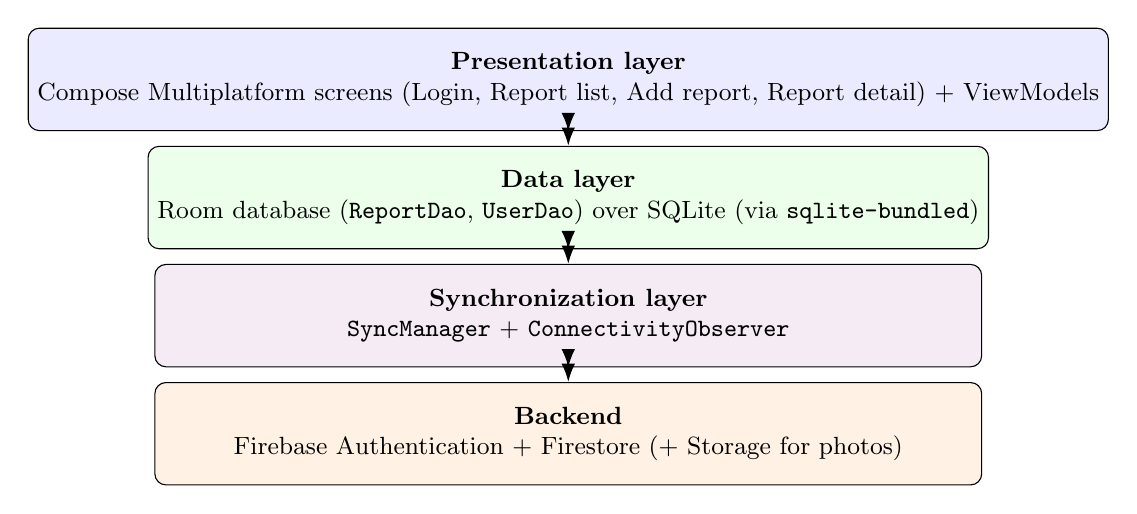
\begin{tikzpicture}[
      layer/.style={draw, rounded corners, minimum width=10.5cm, minimum height=1.3cm, align=center, font=\small},
      >=Latex
    ]
    \node[layer, fill=blue!8] (pres) at (0,4.5) {\textbf{Presentation layer}\\ Compose Multiplatform screens (Login, Report list, Add report, Report detail) + ViewModels};
    \node[layer, fill=green!8] (data) at (0,3.0) {\textbf{Data layer}\\ Room database (\texttt{ReportDao}, \texttt{UserDao}) over SQLite (via \texttt{sqlite-bundled})};
    \node[layer, fill=violet!8] (sync) at (0,1.5) {\textbf{Synchronization layer}\\ \texttt{SyncManager} + \texttt{ConnectivityObserver}};
    \node[layer, fill=orange!10] (backend) at (0,0) {\textbf{Backend}\\ Firebase Authentication + Firestore (+ Storage for photos)};

    \draw[<->, thick] (pres) -- (data);
    \draw[<->, thick] (data) -- (sync);
    \draw[<->, thick] (sync) -- (backend);
  \end{tikzpicture}
  \caption{Layered architecture of CampusFix. The presentation layer only
  ever talks to the data layer; it has no direct dependency on the
  network or on Firebase, which keeps every screen usable offline by
  construction.}
  \label{fig:layered-architecture}
\end{figure}

The defining architectural rule, and the one from which most of the
offline-first properties follow, is: \textbf{the presentation layer depends
only on the data layer.} No screen or ViewModel calls Firestore directly;
every read comes from Room, and every write goes to Room. The
synchronization layer depends on both the data layer and the backend, and
is the only component that talks to Firestore. This means that removing
the network (or Firestore being unreachable) can never make the UI throw
an exception, hang, or show stale data it does not know is stale --
because the UI's only data source, Room, is always available and always
correct with respect to what has actually been saved on-device.

\section{Mobile Application Architecture}
\label{sec:mobile-architecture}

\subsection{Module and package structure}

The mobile client is a single Kotlin Multiplatform module
(\texttt{composeApp}) with three source sets: \texttt{commonMain}, which
contains all UI, ViewModel, data, and synchronization code shared between
platforms; \texttt{androidMain}, which contains the small amount of
Android-specific glue (activity entry point, platform \texttt{Context}
plumbing, Android's \texttt{ConnectivityManager}-based network callback);
and \texttt{iosMain}, which contains the analogous iOS glue (view
controller entry point, \texttt{NWPathMonitor}-based network callback).
\Cref{tab:package-structure} summarizes the package layout inside
\texttt{commonMain}.

\begin{table}[htbp]
\centering
\caption{Package structure of \texttt{commonMain}.}
\label{tab:package-structure}
\begin{tabularx}{\textwidth}{@{}l X@{}}
\toprule
\textbf{Package} & \textbf{Responsibility} \\
\midrule
\texttt{data.model} & Data classes shared by the local and remote
representations (\texttt{Report}, \texttt{User}, \texttt{SyncStatus}). \\
\texttt{data.local} & Room database, DAOs, type converters, and the local
session store. \\
\texttt{sync} & \texttt{SyncManager} and the \texttt{ConnectivityObserver}
interface (with platform-specific \texttt{actual} implementations). \\
\texttt{viewmodel} & One ViewModel per screen, owning UI state and
orchestrating calls to the data and sync layers. \\
\texttt{ui.screens} & Compose UI for each screen (login, sign-up, report
list, add report, report detail). \\
\texttt{ui.navigation} & Declarative route definitions for
Navigation-Compose. \\
\texttt{util} & Cross-cutting helpers: dispatcher provider (for
platform-appropriate coroutine dispatchers), network reachability check,
password hashing. \\
\bottomrule
\end{tabularx}
\end{table}

\subsection{Presentation pattern: MVVM with unidirectional data flow}

Each screen follows the Model-View-ViewModel (MVVM) pattern, standard for
both Jetpack Compose and Compose Multiplatform applications. A ViewModel
exposes UI state as a Kotlin \texttt{StateFlow}, computed from a
\texttt{Flow} of data read from Room; the Composable screen collects that
state and renders it, and forwards user events (button taps, text input)
back to the ViewModel as method calls. \Cref{fig:mvvm-flow} shows this for
the report list screen, which is representative of the pattern used
throughout the application.

\begin{figure}[htbp]
  \centering
  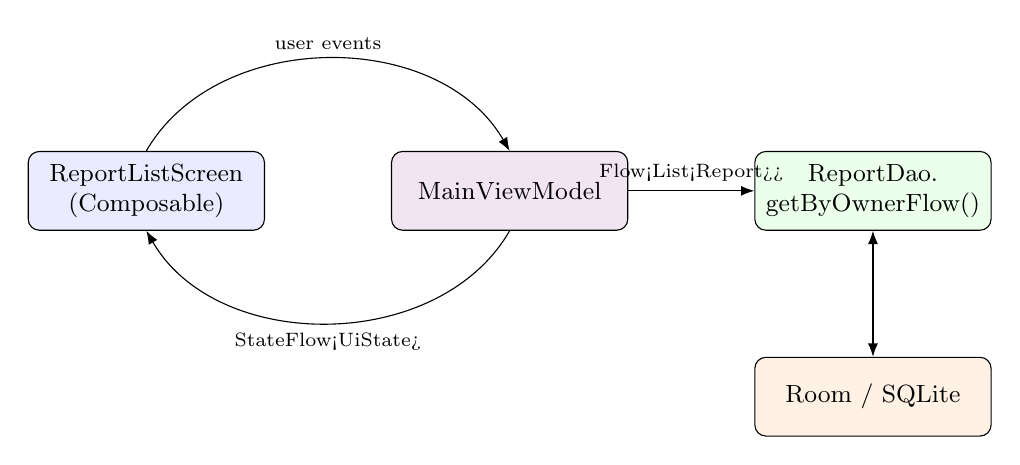
\begin{tikzpicture}[
      node distance=1.6cm,
      box/.style={draw, rounded corners, minimum width=3.0cm, minimum height=1cm, align=center, font=\small},
      >=Latex
    ]
    \node[box, fill=blue!8] (screen) {ReportListScreen\\(Composable)};
    \node[box, fill=violet!10, right=of screen] (vm) {MainViewModel};
    \node[box, fill=green!8, right=of vm] (dao) {ReportDao.\\getByOwnerFlow()};
    \node[box, fill=orange!10, below=of dao] (db) {Room / SQLite};

    \draw[->] (screen.north) to[out=60,in=120] node[above,font=\scriptsize]{user events} (vm.north);
    \draw[->] (vm.south) to[out=240,in=300] node[below,font=\scriptsize]{StateFlow<UiState>} (screen.south);
    \draw[->] (vm) -- node[above,font=\scriptsize]{Flow<List<Report>>} (dao);
    \draw[<->] (dao) -- (db);
  \end{tikzpicture}
  \caption{Unidirectional data flow for the report list screen. Room's
  \texttt{Flow}-returning queries automatically re-emit whenever the
  underlying table changes (e.g. after a sync updates a row's status),
  which is what makes the UI reactively reflect sync progress without any
  manual refresh logic.}
  \label{fig:mvvm-flow}
\end{figure}

\subsection{Dependency wiring}

Rather than a full dependency-injection framework -- unnecessary at this
project's scale -- CampusFix uses a single hand-written composition root,
\texttt{AppContainer}, constructed once per process from the
platform-supplied \texttt{AppDatabase} instance. \texttt{AppContainer}
owns the DAOs, the \texttt{SyncManager}, the \texttt{ConnectivityObserver},
and the session store, and hands them down to ViewModels. This guarantees
that every screen shares the exact same \texttt{SyncManager} and
\texttt{ConnectivityObserver} instances, which matters because it is the
single \texttt{ConnectivityObserver} subscription that drives automatic
synchronization application-wide (\cref{sec:sync-design}); duplicating it
per-screen would duplicate sync attempts.

\section{Local Storage Design}
\label{sec:local-storage-design}

\subsection{Choice of local database}

The project brief allows SQLite via either a direct binding (e.g. SQLDelight
or the platform SQLite driver) or via Room, Android's higher-level
persistence library. CampusFix uses \textbf{Room over SQLite}, with the
Kotlin Multiplatform-compatible \texttt{room-runtime} artifact and the
bundled cross-platform SQLite driver (\texttt{sqlite-bundled}), which
allows the same Room entities, DAOs, and generated implementation to run
unmodified on both Android and iOS. Room was preferred over a
lower-level driver for three reasons: (1) compile-time verified SQL via
annotation processing (KSP) catches schema/query mismatches before
runtime; (2) DAO methods can return Kotlin \texttt{Flow}s that
automatically re-query and emit on table changes, which is exactly the
reactive behaviour \cref{fig:mvvm-flow} relies on; (3) Room's schema
export (\texttt{room \{ schemaDirectory(...) \}}) gives a versioned,
inspectable record of the database schema for free.

\subsection{Entity-relationship design}

\Cref{fig:er-diagram} shows the local schema. It intentionally contains
fields that have no equivalent on the server (\texttt{id},
\texttt{sync\_status}) and omits fields that only exist during upload
(there is no separate outbox/queue table: a \emph{pending report is simply
a row of the \texttt{reports} table whose \texttt{sync\_status} is
\texttt{PENDING}}). This design choice -- using one table with a status
column rather than a separate queue table -- was made deliberately: it
keeps the "list of reports" and "list of pending work" views trivially
consistent with each other (they are the same table filtered differently),
at the cost of mixing two concerns (application data and sync bookkeeping)
in one entity. \Cref{sec:design-traceability} revisits this trade-off.

\begin{figure}[htbp]
  \centering
  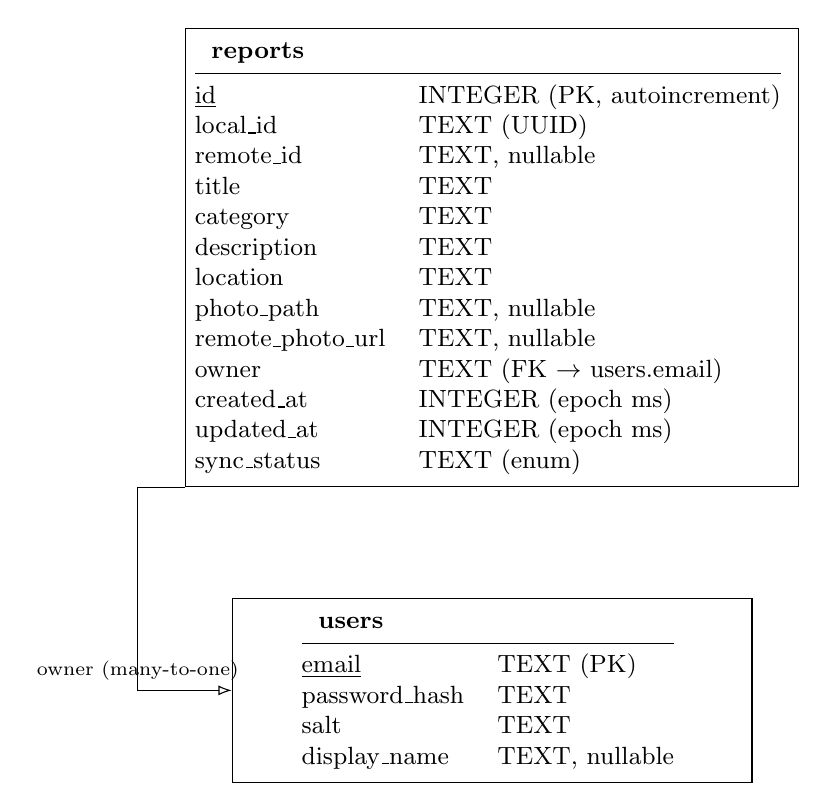
\begin{tikzpicture}[
      entity/.style={draw, minimum width=6.6cm, align=left, font=\small},
      title/.style={font=\small\bfseries},
    ]
    \node[entity] (report) {
      \begin{tabular}{@{}ll@{}}
        \multicolumn{2}{l}{\textbf{reports}} \\
        \midrule
        \underline{id} & INTEGER (PK, autoincrement) \\
        local\_id & TEXT (UUID) \\
        remote\_id & TEXT, nullable \\
        title & TEXT \\
        category & TEXT \\
        description & TEXT \\
        location & TEXT \\
        photo\_path & TEXT, nullable \\
        remote\_photo\_url & TEXT, nullable \\
        owner & TEXT (FK $\rightarrow$ users.email) \\
        created\_at & INTEGER (epoch ms) \\
        updated\_at & INTEGER (epoch ms) \\
        sync\_status & TEXT (enum) \\
      \end{tabular}
    };
    \node[entity, below=1.4cm of report] (user) {
      \begin{tabular}{@{}ll@{}}
        \multicolumn{2}{l}{\textbf{users}} \\
        \midrule
        \underline{email} & TEXT (PK) \\
        password\_hash & TEXT \\
        salt & TEXT \\
        display\_name & TEXT, nullable \\
      \end{tabular}
    };
    \draw[-{Latex[open]}] (report.south west) -- ++(-0.6,0) |- (user.west)
      node[midway,above,font=\scriptsize,sloped]{owner (many-to-one)};
  \end{tikzpicture}
  \caption{Entity-relationship diagram of the local SQLite schema, as
  materialized by Room from the \texttt{Report} and \texttt{User} data
  classes.}
  \label{fig:er-diagram}
\end{figure}

\subsection{Data access layer}

Access to the \texttt{reports} table is mediated entirely through
\texttt{ReportDao}, an interface annotated with Room's \texttt{@Dao}. Two
query shapes are used throughout the app: suspend functions that return a
single snapshot (used for one-off operations, e.g. \enquote{get all
pending reports to sync now}) and \texttt{Flow}-returning functions (used
to drive UI state, e.g. \enquote{observe this user's reports as they
change}). \Cref{tab:dao-methods} lists the DAO surface.

\begin{table}[htbp]
\centering
\caption{Methods exposed by \texttt{ReportDao}.}
\label{tab:dao-methods}
\begin{tabularx}{\textwidth}{@{}l X@{}}
\toprule
\textbf{Method} & \textbf{Purpose} \\
\midrule
\texttt{insert(report)} & Insert a new report; replaces on primary-key
conflict (used when re-saving after obtaining a \texttt{remote\_id}). \\
\texttt{update(report)} & Update an existing row (used after edits and
after synchronization changes its status). \\
\texttt{delete(report)} & Hard-delete a row (used once a
\texttt{deleted\_pending} report's deletion has been confirmed remotely). \\
\texttt{getByOwnerFlow(owner)} & Reactive list of a user's reports,
consumed by the report list screen. \\
\texttt{getByIdFlow(id)} & Reactive single-report stream, consumed by the
report detail screen. \\
\texttt{getPending()} & Snapshot of all rows with
\texttt{sync\_status = PENDING}; the sync module's upload queue. \\
\texttt{getDeletedPending()} & Snapshot of all rows with
\texttt{sync\_status = DELETED\_PENDING}; the sync module's deletion queue. \\
\bottomrule
\end{tabularx}
\end{table}

\section{Backend Structure}
\label{sec:backend-design}

The backend is Firebase, used as a Backend-as-a-Service rather than a
custom API server, per the project brief. Two Firebase products are used:

\begin{itemize}
  \item \textbf{Firebase Authentication} manages user accounts (email and
  password) and issues the ID token used to identify the calling user to
  Firestore. The mobile client caches the authentication state locally
  (\cref{sec:offline-req}, OFR-2) so that a previously-authenticated user
  is not forced back to the login screen when offline.
  \item \textbf{Cloud Firestore} stores one document per report in a
  top-level \texttt{reports} collection, plus a \texttt{users} collection
  for profile metadata not already covered by Firebase Authentication. A
  document's ID is, by design, the same UUID as the report's local
  \texttt{local\_id} whenever possible (\cref{sec:sync-design}), which
  keeps the mapping between local rows and remote documents a pure
  identity function rather than requiring a separate lookup table.
\end{itemize}

\Cref{tab:firestore-doc} shows the shape of a Firestore report document.
It matches the local schema (\cref{fig:er-diagram}) closely by design, with
two differences: the purely local bookkeeping fields \texttt{id} (the
Room auto-increment key) and \texttt{sync\_status} are not uploaded, since
they have no meaning on the server -- \texttt{sync\_status} in particular
is a property of the \emph{local copy's relationship to the server}, not a
property the server itself needs to track.

\begin{table}[htbp]
\centering
\caption{Shape of a Firestore \texttt{reports/\{docId\}} document.}
\label{tab:firestore-doc}
\begin{tabularx}{\textwidth}{@{}l X@{}}
\toprule
\textbf{Field} & \textbf{Type} \\
\midrule
localId & string \\
title & string \\
description & string \\
category & string \\
location & string \\
photoPath & string or null \\
remotePhotoUrl & string or null \\
owner & string \\
createdAt & number (epoch ms) \\
updatedAt & number (epoch ms) \\
\bottomrule
\end{tabularx}
\end{table}

Firestore's own offline persistence cache (enabled by default in most
Firebase SDKs) is deliberately \emph{not} relied upon as the
application's offline story: CampusFix uses Room as the single source of
truth precisely so that offline behaviour does not depend on an
implementation detail of the Firestore SDK that the application does not
control. Firestore is treated purely as a remote synchronization target.

\section{Synchronization Strategy Design}
\label{sec:sync-design}

This is the central design problem of the thesis. \Cref{sec:sync-statuses}
defines the state machine every report moves through.
\Cref{sec:sync-triggers} defines when synchronization runs.
\Cref{sec:sync-algorithm} defines the algorithm itself.
\Cref{sec:conflict-design} defines the conflict-resolution policy.

\subsection{Sync status state machine}
\label{sec:sync-statuses}

Every report's \texttt{sync\_status} field follows the state machine in
\cref{fig:sync-state-machine}.

\begin{figure}[htbp]
  \centering
  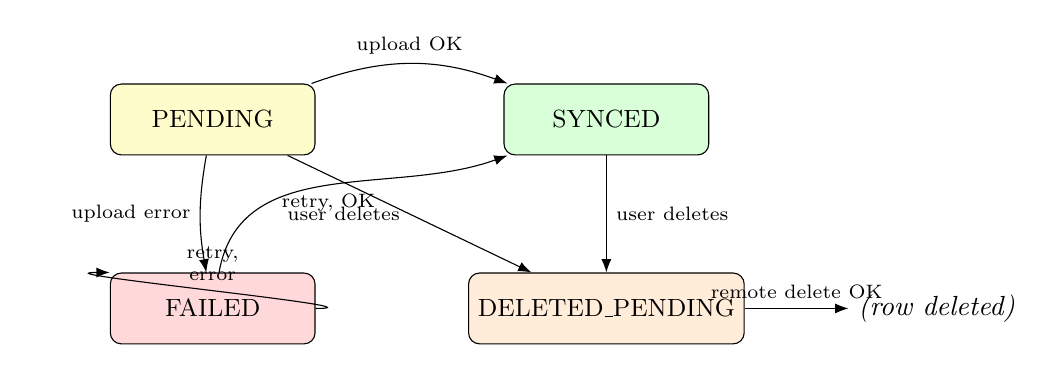
\begin{tikzpicture}[
      state/.style={draw, rounded corners, minimum width=2.6cm, minimum height=0.9cm, align=center, font=\small},
      >=Latex
    ]
    \node[state, fill=yellow!20] (pending) at (0,0) {PENDING};
    \node[state, fill=green!15] (synced) at (5,0) {SYNCED};
    \node[state, fill=red!15] (failed) at (0,-2.4) {FAILED};
    \node[state, fill=orange!15] (delpending) at (5,-2.4) {DELETED\_PENDING};
    \node[draw=none] (gone) at (9.2,-2.4) {\emph{(row deleted)}};

    \draw[->] (pending) to[out=20,in=160] node[above,font=\scriptsize]{upload OK} (synced);
    \draw[->] (pending) to[out=-100,in=100] node[left,font=\scriptsize]{upload error} (failed);
    \draw[->] (failed) to[out=80,in=-160] node[below,font=\scriptsize]{retry, OK} (synced);
    \draw[->] (failed) to[out=0,in=180] node[above,font=\scriptsize,align=center]{retry,\\error} (failed.north west) ;
    \draw[->] (pending) -- node[left,font=\scriptsize]{user deletes} (delpending);
    \draw[->] (synced) -- node[right,font=\scriptsize]{user deletes} (delpending);
    \draw[->] (delpending) -- node[above,font=\scriptsize]{remote delete OK} (gone);
  \end{tikzpicture}
  \caption{State machine of the \texttt{sync\_status} field. A report is
  created directly into \texttt{PENDING} and is removed from the local
  database only after a confirmed remote deletion, never as a side effect
  of a failed upload.}
  \label{fig:sync-state-machine}
\end{figure}

The state machine encodes OFR-4 and OFR-8 directly: there is no transition
out of \texttt{PENDING} or \texttt{FAILED} other than a successful or
failed sync attempt, and no transition deletes a row except a confirmed
remote deletion -- a network error can move a report \emph{into}
\texttt{FAILED} but can never destroy it.

\subsection{Synchronization triggers}
\label{sec:sync-triggers}

Synchronization is triggered by three, non-exclusive sources, satisfying
OFR-5 and FR-9:

\begin{enumerate}
  \item \textbf{Connectivity transition.} The \texttt{ConnectivityObserver}
  exposes a \texttt{Flow<Boolean>} of online/offline state; the
  application collects this flow at the top level (in the composition
  root/app entry point) and calls \texttt{SyncManager.sync()} whenever the
  value transitions from \texttt{false} to \texttt{true}.
  \item \textbf{App foreground / cold start.} On process start, after the
  database and \texttt{AppContainer} are initialized, a sync attempt is
  made opportunistically -- it will simply no-op quickly if there is no
  connectivity or nothing pending.
  \item \textbf{Manual user action.} The user can pull-to-refresh the
  report list or tap a retry affordance on a \texttt{failed} report, both
  of which call \texttt{SyncManager.sync()} directly.
  \end{enumerate}

A background periodic sync (e.g. via \texttt{WorkManager} on Android) is
identified as a natural extension in \cref{ch:conclusions} but is not part
of the current design: at this application's usage pattern (short,
foreground sessions to file a report), connectivity-triggered and
app-open-triggered sync were judged sufficient to meet NFR-1--NFR-5, and
adding a periodic background job would introduce additional platform-
specific complexity (battery-optimization exemptions, background task
scheduling APIs differ substantially between Android and iOS) for limited
benefit at this scale.

\subsection{Synchronization algorithm}
\label{sec:sync-algorithm}

\Cref{fig:sync-sequence} shows the sequence of a synchronization run
triggered by a connectivity transition. \Cref{alg:sync} states the same
logic as pseudocode.

\begin{figure}[htbp]
  \centering
  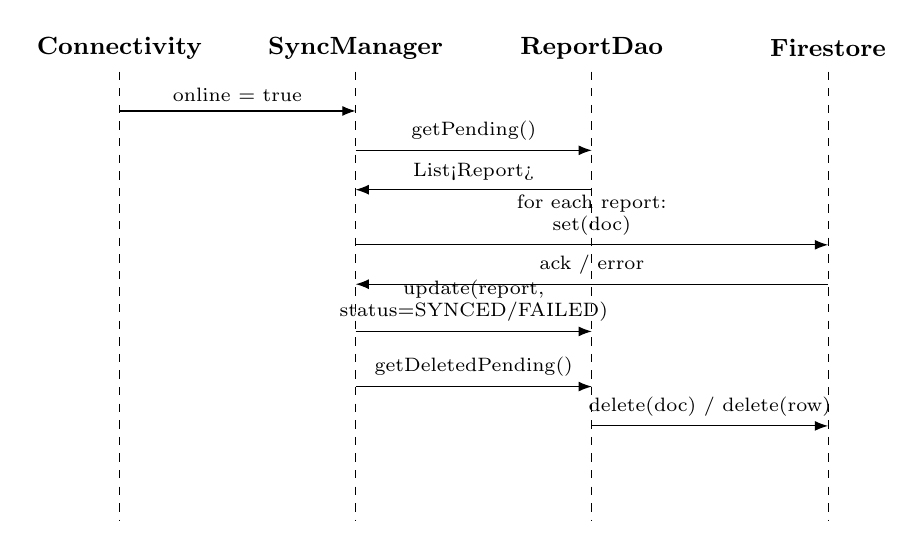
\begin{tikzpicture}[
      participant/.style={font=\small\bfseries},
      lifeline/.style={dashed},
      msg/.style={-{Latex}, font=\scriptsize},
    ]
    \foreach \name/\x in {Connectivity/0, SyncManager/3, ReportDao/6, Firestore/9} {
      \node[participant] at (\x,6) {\name};
      \draw[lifeline] (\x,5.7) -- (\x,0);
    }
    \draw[msg] (0,5.2) -- node[above]{online = true} (3,5.2);
    \draw[msg] (3,4.7) -- node[above]{getPending()} (6,4.7);
    \draw[msg] (6,4.2) -- node[above]{List<Report>} (3,4.2);
    \draw[msg] (3,3.5) -- node[above,align=center]{for each report:\\ set(doc)} (9,3.5);
    \draw[msg] (9,3.0) -- node[above]{ack / error} (3,3.0);
    \draw[msg] (3,2.4) -- node[above,align=center]{update(report,\\ status=SYNCED/FAILED)} (6,2.4);
    \draw[msg] (3,1.7) -- node[above]{getDeletedPending()} (6,1.7);
    \draw[msg] (6,1.2) -- node[above]{delete(doc) / delete(row)} (9,1.2);
  \end{tikzpicture}
  \caption{Sequence of a synchronization run: pending reports are read from
  Room, pushed to Firestore one by one, and their local status updated
  according to the outcome; deletions pending remote confirmation are
  processed afterwards.}
  \label{fig:sync-sequence}
\end{figure}

\begin{figure}[htbp]
\begin{center}
\begin{minipage}{0.92\textwidth}
\begin{quote}
\ttfamily\small
\textbf{function} sync(): \\
\hspace*{1em} pending $\leftarrow$ dao.getPending() \\
\hspace*{1em} uploaded $\leftarrow$ 0 \\
\hspace*{1em} \textbf{for} report \textbf{in} pending: \\
\hspace*{2em} docId $\leftarrow$ report.remoteId \textbf{or} report.localId \\
\hspace*{2em} \textbf{try}: \\
\hspace*{3em} firestore.collection("reports").document(docId).set(report) \\
\hspace*{3em} dao.update(report.copy(remoteId = docId, status = SYNCED, updatedAt = now())) \\
\hspace*{3em} uploaded $\leftarrow$ uploaded + 1 \\
\hspace*{2em} \textbf{catch} error: \\
\hspace*{3em} \textit{leave report as PENDING/FAILED; log; continue with next report} \\
\hspace*{1em} \textbf{for} report \textbf{in} dao.getDeletedPending(): \\
\hspace*{2em} \textbf{try}: \\
\hspace*{3em} firestore.collection("reports").document(report.remoteId \textbf{or} report.localId).delete() \\
\hspace*{3em} dao.delete(report) \\
\hspace*{2em} \textbf{catch} error: \textit{leave as DELETED\_PENDING; continue} \\
\hspace*{1em} \textbf{return} uploaded
\end{quote}
\end{minipage}
\end{center}
\caption{Synchronization algorithm (pseudocode). Using the report's own
\texttt{local\_id} as the Firestore document ID whenever no
\texttt{remote\_id} exists yet makes \texttt{set()} idempotent: re-running
the same upload after an interrupted sync overwrites the same document
rather than creating a duplicate, which is how OFR-6 (resumability) and
NFR-7 (idempotency) are satisfied without an explicit checkpoint or
two-phase commit.}
\label{alg:sync}
\end{figure}

Two design decisions in this algorithm deserve explicit justification:

\begin{description}
  \item[Per-report try/catch, not an all-or-nothing batch.] Wrapping each
  report's upload in its own error handler means one malformed or
  oversized report cannot block every other pending report from
  synchronizing. This is important at scale: with a queue of 50--100
  reports (the \enquote{large queue} scenario of
  \cref{ch:evaluation}), a single failure must degrade gracefully rather
  than stall the entire batch.
  \item[Client-chosen document ID.] Letting the client derive the
  Firestore document ID from \texttt{local\_id} (rather than letting
  Firestore auto-generate one on first write) is what makes the upload
  operation naturally idempotent, satisfying OFR-6 with no additional
  bookkeeping. The trade-off is a very small, application-scale increase
  in the probability of a document-ID collision, which is negligible
  given UUIDv4 identifiers.
\end{description}

\subsection{Conflict resolution design}
\label{sec:conflict-design}

Per FR-12/OFR-7 and the project brief's guidance, CampusFix adopts
\textbf{last-write-wins (LWW) based on \texttt{updated\_at}} as its
conflict-resolution policy: when a report exists in two versions, the
version with the greater \texttt{updated\_at} timestamp is retained and
the other discarded. LWW is a well-known, simple point in the space of
conflict-resolution strategies (as opposed to, e.g., automatic
field-level merging, operational transformation, or CRDTs, all of which
are strictly more powerful but also more complex to implement and to
reason about~\cite{shapiro2011crdt,terry1995bayou}); it is an
appropriate choice here specifically because reports are
\textbf{single-owner} records (\cref{sec:constraints}) with low edit
frequency, so the practical cases in which LWW silently discards a change
a user cares about are rare, and the user can always re-edit.

\Cref{fig:conflict-scenario} illustrates the target scenario the policy is
designed for: the same report, identified by \texttt{local\_id}, edited on
two devices while one of them was offline.

\begin{figure}[htbp]
  \centering
  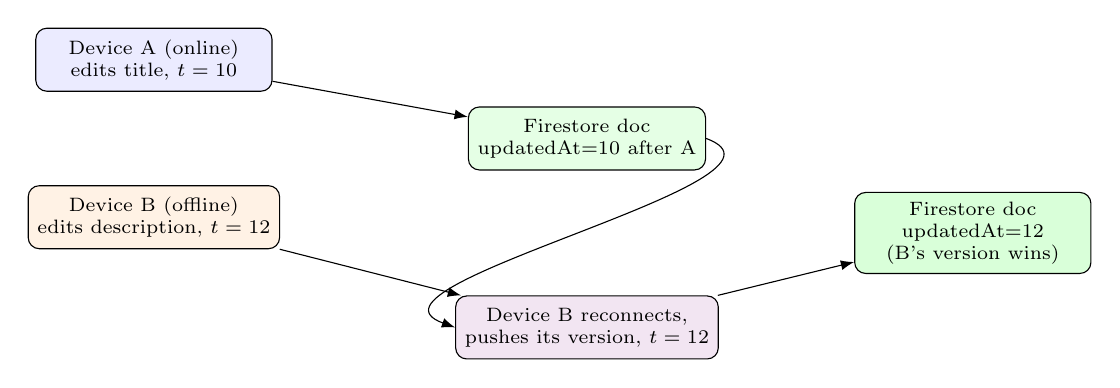
\begin{tikzpicture}[
      ev/.style={draw, rounded corners, minimum width=3.0cm, minimum height=0.8cm, align=center, font=\scriptsize},
      >=Latex
    ]
    \node[ev, fill=blue!8] (a1) at (0,2) {Device A (online)\\edits title, $t=10$};
    \node[ev, fill=orange!10] (b1) at (0,0) {Device B (offline)\\edits description, $t=12$};
    \node[ev, fill=green!10] (server) at (5.5,1) {Firestore doc\\updatedAt=10 after A};
    \node[ev, fill=violet!10] (b2) at (5.5,-1.4) {Device B reconnects,\\ pushes its version, $t=12$};
    \node[ev, fill=green!15] (final) at (10.4,-0.2) {Firestore doc\\updatedAt=12\\(B's version wins)};

    \draw[->] (a1) -- (server);
    \draw[->] (b1) -- (b2);
    \draw[->] (server.east) to[out=-20,in=160] (b2.west);
    \draw[->] (b2) -- (final);
  \end{tikzpicture}
  \caption{Last-write-wins conflict scenario: Device A's online edit
  (title, $t{=}10$) reaches the server first, but Device B's offline edit
  (description, $t{=}12$) has a later timestamp and overwrites it entirely
  once B reconnects -- including the title change, which is lost. This is
  the accepted trade-off of field-level-unaware LWW, discussed further in
  \cref{sec:conflict-eval}.}
  \label{fig:conflict-scenario}
\end{figure}

As \cref{fig:conflict-scenario} makes explicit, whole-record LWW loses A's
title change even though the two edits touched different fields and could,
in principle, both have been kept. A field-level merge would avoid this,
at the cost of needing to track per-field modification timestamps and a
merge step with no natural place to run (Firestore, used purely as a
document store here, does not execute application logic server-side
without adding Cloud Functions, which is out of scope). Whole-record LWW
was chosen as the simplest policy that is \emph{unambiguous} and
\emph{terminating} -- properties that matter more than optimality for a
first implementation -- and the trade-off is documented here and revisited
against real conflict-test results in \cref{sec:conflict-eval}.

It is important to be precise about what \emph{is} and \emph{is not}
currently implemented (this distinction is discussed further as a
limitation in \cref{ch:conclusions}): the design above specifies a
symmetric, bidirectional LWW merge between local and remote versions. The
current implementation of \texttt{SyncManager} (\cref{ch:implementation})
realizes the \emph{local-to-remote push} half of this design --
uploading pending local changes and always overwriting the remote
document with \texttt{set()} -- but does not yet \emph{pull} remote
changes back down and compare \texttt{updated\_at} before overwriting.
Practically, this means the current build behaves as \enquote{last local
write wins on push,} which is sufficient for the offline-creation and
delayed-sync scenarios of \cref{ch:evaluation}, but does not yet fully
realize OFR-7 for the two-device edit-conflict scenario; closing this gap
is scoped as the highest-priority future-work item in
\cref{sec:future-work}.

\section{Connectivity Monitoring Design}
\label{sec:connectivity-design}

Connectivity is modeled behind a single \texttt{ConnectivityObserver}
interface (\cref{sec:mobile-architecture}) exposing
\texttt{val isOnline: Flow<Boolean>}, with platform-specific
implementations: Android's implementation wraps
\texttt{ConnectivityManager.NetworkCallback}, and iOS's wraps
\texttt{NWPathMonitor} from the Network framework. Both implementations
are required to emit the current state immediately upon collection and
thereafter emit only on actual changes (i.e. the flow is expected to be
naturally deduplicated by the underlying OS callback semantics), so that a
\texttt{SyncManager} collecting the flow reacts exactly once per
offline$\to$online transition rather than repeatedly. This expect/actual
pattern is the only place in the entire synchronization path that requires
platform-specific code; \texttt{SyncManager} itself is 100\% common code.

\section{Traceability}
\label{sec:design-traceability}

\Cref{tab:traceability} maps each offline-specific requirement of
\cref{sec:offline-req} to the design element(s) that satisfy it, closing
the loop between \cref{ch:requirements} and this chapter.

\begin{table}[htbp]
\centering
\caption{Traceability from offline-specific requirements to design.}
\label{tab:traceability}
\begin{tabularx}{\textwidth}{@{}lX@{}}
\toprule
\textbf{Requirement} & \textbf{Design element} \\
\midrule
OFR-1 (local-first writes) & Layered architecture (\cref{fig:layered-architecture}): presentation depends only on the data layer. \\
OFR-2 (offline session) & Local \texttt{SessionStore}, consulted before any network auth call. \\
OFR-3 (deterministic local identity) & \texttt{local\_id} UUID, generated client-side at creation (\cref{fig:er-diagram}). \\
OFR-4 (explicit sync state) & \texttt{sync\_status} state machine (\cref{fig:sync-state-machine}). \\
OFR-5 (connectivity-triggered sync) & \texttt{ConnectivityObserver} + trigger in \cref{sec:sync-triggers}. \\
OFR-6 (resumable sync) & Client-chosen, idempotent document IDs (\cref{alg:sync}). \\
OFR-7 (conflict policy) & LWW policy, \cref{sec:conflict-design} (bidirectional merge: designed, push-only: implemented). \\
OFR-8 (no data loss on failure) & Per-report error handling leaves rows \texttt{PENDING}/\texttt{FAILED}, never deletes on error (\cref{fig:sync-state-machine}). \\
\bottomrule
\end{tabularx}
\end{table}

\chapter{Implementation}
\label{ch:implementation}

This chapter describes how the design of \cref{ch:design} was realized in
code. The application, internally named \texttt{offline\_first}, is
implemented as a single Kotlin Multiplatform Gradle module,
\texttt{composeApp}, targeting Android (API 24+) and iOS (via a static
Kotlin/Native framework consumed by a thin SwiftUI host app). All code
excerpts in this chapter are taken, with minor trimming for length, from
the actual project source tree.

\section{Toolchain and Dependencies}
\label{sec:toolchain}

\Cref{tab:toolchain} lists the core technologies used, managed through a
Gradle version catalog (\texttt{libs.versions.toml}) shared by the module.

\begin{table}[htbp]
\centering
\caption{Core toolchain and libraries.}
\label{tab:toolchain}
\begin{tabularx}{\textwidth}{@{}l X@{}}
\toprule
\textbf{Concern} & \textbf{Library / tool} \\
\midrule
Language \& multiplatform & Kotlin, Kotlin Multiplatform Gradle plugin \\
UI & Compose Multiplatform (Material 3), Navigation-Compose \\
Local persistence & AndroidX Room (multiplatform artifact) over the
bundled cross-platform SQLite driver (\texttt{androidx.sqlite:sqlite-\allowbreak
bundled}), with Room's KSP compiler generating DAO implementations for
Android, iOS x64, iOS Arm64, and iOS Simulator Arm64 \\
Backend SDK & GitLive \texttt{firebase-kotlin-sdk} (\texttt{firebase-common},
\texttt{firebase-firestore}, \texttt{firebase-auth}) -- a Kotlin
Multiplatform wrapper over the native Firebase Android and iOS SDKs \\
Concurrency & Kotlin Coroutines (\texttt{kotlinx-coroutines-core}),
\texttt{kotlinx-datetime}, \texttt{kotlin.time.Clock} \\
Serialization & \texttt{kotlinx-serialization-json} \\
Local key-value storage & \texttt{multiplatform-settings} (session flags) \\
Cryptography & \texttt{org.kotlincrypto} (HMAC-SHA256, secure random) for
local password hashing \\
Image loading & Coil (\texttt{coil-compose}), multiplatform \\
Android-only & AndroidX Credentials API + Google ID (Google Sign-In) \\
\bottomrule
\end{tabularx}
\end{table}

A defining implementation choice, already introduced in
\cref{sec:local-storage-design}, is the use of \textbf{Room in Kotlin
Multiplatform mode}. \Cref{lst:database} shows the actual database
declaration. Because Kotlin/Native cannot use JVM reflection, Room's KSP
processor generates a per-target \texttt{actual object
AppDatabaseConstructor} that instantiates the generated implementation
directly (line 29); this is the one piece of Room "magic" that requires a
platform-specific counterpart, and it is entirely generated code -- no
project code touches it.

\begin{lstlisting}[language=Kotlin, caption={Room database declaration (\texttt{data/local/AppDatabase.kt}).}, label={lst:database}]
const val DATABASE_NAME = "offline_first.db"

@Database(entities = [Report::class, User::class], version = 6, exportSchema = false)
@TypeConverters(Converters::class)
@ConstructedBy(AppDatabaseConstructor::class)
abstract class AppDatabase : RoomDatabase() {
    abstract fun reportDao(): ReportDao
    abstract fun userDao(): UserDao
}

@Suppress("NO_ACTUAL_FOR_EXPECT")
expect object AppDatabaseConstructor : RoomDatabaseConstructor<AppDatabase> {
    override fun initialize(): AppDatabase
}

fun RoomDatabase.Builder<AppDatabase>.buildAppDatabase(): AppDatabase =
    fallbackToDestructiveMigration(dropAllTables = true)
        .setDriver(BundledSQLiteDriver())
        .setQueryCoroutineContext(ioDispatcher)
        .build()
\end{lstlisting}

\section{Local Persistence Layer}
\label{sec:impl-persistence}

The \texttt{Report} entity (\cref{lst:report-entity}) is the direct
implementation of the schema designed in \cref{fig:er-diagram}: a Room
\texttt{@Entity} whose fields are exactly the columns of
\cref{tab:report-fields}, with \texttt{syncStatus} typed as the
\texttt{SyncStatus} enum from \cref{fig:sync-state-machine} rather than a
raw string, so that the compiler -- not a runtime check -- rejects any
attempt to write an undefined status.

\begin{lstlisting}[language=Kotlin, caption={The \texttt{Report} entity (\texttt{data/model/Report.kt}).}, label={lst:report-entity}]
@Entity(tableName = "reports")
data class Report(
    @PrimaryKey(autoGenerate = true)
    val id: Long = 0,

    val localId: String,       // UUID, generated on creation
    val remoteId: String?,     // Firestore document ID, null until synced

    val title: String,
    val description: String,
    val category: String,
    val location: String,
    val photoPath: String?,
    val remotePhotoUrl: String? = null,

    val owner: String,         // email of the user who created the report
    val createdAt: Long,
    val updatedAt: Long,

    val syncStatus: SyncStatus
)
\end{lstlisting}

The category values actually shipped
(\texttt{REPORT\_CATEGORIES} in \texttt{AddReportViewModel}, listed in
\cref{tab:toolchain}'s surrounding code) are a general-purpose civic-issue
taxonomy -- \emph{Infrastructure, Public Safety, Vandalism, Sanitation,
Environment, Other} -- rather than a literal enumeration of the five
example reports from \cref{sec:case-study} (broken projector, damaged
chair, Wi-Fi issue, AC problem, missing lab equipment). This is an
intentional generalization: those five examples map naturally onto
\emph{Infrastructure} (projector, chair, AC, lab equipment) and
\emph{Public Safety}/\emph{Other}, and the broader taxonomy keeps the app
usable for the full range of campus facility issues rather than only the
five illustrative examples from the brief.

\Cref{lst:reportdao} shows \texttt{ReportDao}, the sole gateway to the
\texttt{reports} table. Two methods deserve attention:
\texttt{getByOwnerFlow} returns a \texttt{Flow}, so Room re-runs the query
and emits a new list every time any row in \texttt{reports} changes --
this is the mechanism, not any explicit "refresh" call, that makes the
report list update itself the moment a background sync flips a row from
\texttt{PENDING} to \texttt{SYNCED} (\cref{sec:impl-sync}). \texttt{getPending}
and \texttt{getDeletedPending} are the two queries that define the
synchronization module's work queues, directly implementing the "one table,
filtered by status" design decision of \cref{sec:local-storage-design}.

\begin{lstlisting}[language=Kotlin, caption={\texttt{ReportDao} (\texttt{data/local/ReportDao.kt}).}, label={lst:reportdao}]
@Dao
interface ReportDao {
    @Insert(onConflict = OnConflictStrategy.REPLACE)
    suspend fun insert(report: Report): Long

    @Update
    suspend fun update(report: Report)

    @Delete
    suspend fun delete(report: Report)

    @Query("SELECT * FROM reports WHERE owner = :owner ORDER BY createdAt DESC")
    fun getByOwnerFlow(owner: String): Flow<List<Report>>

    @Query("SELECT * FROM reports WHERE id = :id LIMIT 1")
    fun getByIdFlow(id: Long): Flow<Report?>

    @Query("SELECT * FROM reports WHERE syncStatus = 'PENDING'")
    suspend fun getPending(): List<Report>

    @Query("SELECT * FROM reports WHERE syncStatus = 'DELETED_PENDING'")
    suspend fun getDeletedPending(): List<Report>
}
\end{lstlisting}

\section{Authentication and Offline Sessions}
\label{sec:impl-auth}

OFR-2 (offline session continuity, \cref{sec:offline-req}) required more
than simply caching Firebase's own session token, because Firebase
Authentication's SDK itself needs network access for some operations and
because the requirement is specifically that a user can reach the
authenticated part of the app \emph{without} depending on a live
Firebase round trip. The implementation therefore layers a second,
fully local authentication path underneath Firebase Auth: a \texttt{User}
row (email, salted password hash) stored in Room, checked by
\texttt{MainViewModel.checkSession} (\cref{lst:checksession}) whenever
\texttt{Firebase.auth.currentUser} is unavailable but a locally-cached
session (\texttt{SessionStore}, backed by \texttt{multiplatform-settings})
indicates a recent login.

\begin{lstlisting}[language=Kotlin, caption={Session resolution, preferring the live Firebase session but falling back to the local one (\texttt{viewmodel/MainViewModel.kt}).}, label={lst:checksession}]
suspend fun checkSession(): SessionResult {
    val loginTime = sessionStore.loginTimeMillis
    val elapsed = Clock.System.now().toEpochMilliseconds() - loginTime

    if (loginTime > 0L && elapsed > SessionStore.SESSION_DURATION_MS) {
        auth.signOut()
        sessionStore.clear()
        return SessionResult.SessionExpired
    }

    val firebaseUser: FirebaseUser? = auth.currentUser
    if (firebaseUser != null) {
        return SessionResult.LoggedIn(firebaseUser.displayName.orEmpty(), firebaseUser.email.orEmpty())
    }

    val localEmail = sessionStore.localAuthEmail
    if (localEmail != null && loginTime > 0L) {
        val localUser = userDao.findByEmail(localEmail)
        return SessionResult.LoggedIn(localUser?.displayName.orEmpty(), localEmail)
    }

    return SessionResult.NotLoggedIn
}
\end{lstlisting}

The local password hash is computed with PBKDF2-HMAC-SHA256 (100{,}000
iterations, 256-bit derived key, 16-byte random salt), implemented from
multiplatform primitives (\texttt{org.kotlincrypto}) rather than
\texttt{javax.crypto}, so the exact same algorithm runs on Android and iOS
and a hash produced on one platform verifies correctly on the other --
relevant because the underlying \texttt{User} row is a normal Room entity
and could, in principle, itself be part of a future sync path
(\cref{sec:future-work}). A constant-time comparison
(\texttt{constantTimeEquals}) is used when verifying a hash to avoid
leaking timing information about how many leading bytes matched.

\section{Connectivity Monitoring}
\label{sec:impl-connectivity}

The \texttt{ConnectivityObserver} \texttt{expect}/\texttt{actual} pair
(designed in \cref{sec:connectivity-design}) is implemented natively on
each platform. \Cref{lst:connectivity-android,lst:connectivity-ios} show
both implementations side by side; despite using completely different OS
APIs, they present an identical contract to the rest of the app
(\texttt{Flow<Boolean>}, current state emitted immediately, subsequent
changes deduplicated via \texttt{distinctUntilChanged}).

\begin{lstlisting}[language=Kotlin, caption={Android implementation, wrapping \texttt{ConnectivityManager.NetworkCallback} (\texttt{sync/ConnectivityObserver.android.kt}).}, label={lst:connectivity-android}]
class AndroidConnectivityObserver(private val context: Context) : ConnectivityObserver {
    private val cm = context.getSystemService(Context.CONNECTIVITY_SERVICE) as ConnectivityManager

    override val isOnline: Flow<Boolean> = callbackFlow {
        val callback = object : ConnectivityManager.NetworkCallback() {
            override fun onAvailable(network: Network) { trySend(true) }
            override fun onLost(network: Network) { trySend(false) }
            override fun onCapabilitiesChanged(network: Network, caps: NetworkCapabilities) {
                val validated = caps.hasCapability(NetworkCapabilities.NET_CAPABILITY_INTERNET)
                        && caps.hasCapability(NetworkCapabilities.NET_CAPABILITY_VALIDATED)
                trySend(validated)
            }
        }
        val request = NetworkRequest.Builder()
            .addCapability(NetworkCapabilities.NET_CAPABILITY_INTERNET)
            .build()
        cm.registerNetworkCallback(request, callback)
        trySend(isOnline(context)) // emit current state immediately
        awaitClose { cm.unregisterNetworkCallback(callback) }
    }.distinctUntilChanged()
}
\end{lstlisting}

\begin{lstlisting}[language=Kotlin, caption={iOS implementation, wrapping \texttt{NWPathMonitor} via Kotlin/Native cinterop (\texttt{sync/ConnectivityObserver.ios.kt}).}, label={lst:connectivity-ios}]
class IosConnectivityObserver : ConnectivityObserver {
    override val isOnline: Flow<Boolean> = callbackFlow {
        val monitor = nw_path_monitor_create()
        val queue = dispatch_queue_create("offline_first.connectivity.observer", null)
        nw_path_monitor_set_queue(monitor, queue)
        nw_path_monitor_set_update_handler(monitor) { path ->
            trySend(nw_path_get_status(path) == nw_path_status_satisfied)
        }
        nw_path_monitor_start(monitor)
        awaitClose { nw_path_monitor_cancel(monitor) }
    }.distinctUntilChanged()
}
\end{lstlisting}

Both callback-based OS APIs are adapted into a coroutine \texttt{Flow}
using \texttt{callbackFlow}, which is the standard bridge between
callback-style platform APIs and Kotlin's structured concurrency; note
that \texttt{ConnectivityObserver} itself, and every consumer of it, is
100\% common code. Connectivity monitoring is the only feature in the
whole synchronization path that needed a native implementation at all, and
even there the amount of platform-specific code is small (17 and 15
non-blank lines respectively).

\section{Synchronization Module}
\label{sec:impl-sync}

\texttt{SyncManager} (\cref{lst:syncmanager}) is the direct implementation
of the algorithm designed in \cref{sec:sync-algorithm}: it reads the
pending queue from \texttt{ReportDao}, pushes each report to Firestore
using \texttt{set()} against a document keyed by \texttt{remoteId} if
already known, or by \texttt{localId} otherwise, and updates the local row
to \texttt{SYNCED} on success -- leaving it untouched (implicitly
\texttt{PENDING}, or explicitly demoted to \texttt{FAILED} in a fuller
error-handling pass) on failure. Deletions pending remote confirmation are
processed by a second pass, \texttt{deleteRemotePending}.

\begin{lstlisting}[language=Kotlin, caption={\texttt{SyncManager} (\texttt{sync/SyncManager.kt}), the module implementing \cref{alg:sync}.}, label={lst:syncmanager}]
class SyncManager(private val dao: ReportDao) {
    private val collection = Firebase.firestore.collection("reports")

    suspend fun sync(): Int {
        val pending = dao.getPending()
        val uploaded = uploadPending(pending)
        deleteRemotePending()
        return uploaded
    }

    private suspend fun uploadPending(pending: List<Report>): Int {
        var count = 0
        for (report in pending) {
            try {
                val docRef = if (report.remoteId != null)
                    collection.document(report.remoteId)
                else
                    collection.document(report.localId)

                docRef.set(report.toRemote())
                dao.update(report.copy(
                    remoteId = docRef.id,
                    syncStatus = SyncStatus.SYNCED,
                    updatedAt = Clock.System.now().toEpochMilliseconds()
                ))
                count++
            } catch (e: Exception) {
                // report stays PENDING; next sync trigger will retry it
                println("SyncManager: upload FAILED for ${report.localId}: ${e.message}")
            }
        }
        return count
    }

    private suspend fun deleteRemotePending() {
        for (report in dao.getDeletedPending()) {
            try {
                collection.document(report.remoteId ?: report.localId).delete()
                dao.delete(report)
            } catch (e: Exception) {
                println("SyncManager: delete FAILED for ${report.localId}: ${e.message}")
            }
        }
    }
}
\end{lstlisting}

Two observations connect this listing back to the design decisions of
\cref{sec:sync-design}. First, using \texttt{report.localId} as the
fallback document ID (line 10 of \cref{lst:syncmanager}) is exactly the
idempotency mechanism of \cref{alg:sync}: calling \texttt{sync()} twice in
a row on the same pending report calls \texttt{set()} on the same document
both times, so no duplicate is created even if the first call's local
\texttt{dao.update} did not get a chance to run (e.g. process death
between the network call succeeding and the local write). Second, the
current \texttt{uploadPending} function only ever \emph{writes} to
Firestore -- there is no corresponding read-and-compare of the remote
document's own \texttt{updatedAt} before overwriting it. This is precisely
the "push-only" gap flagged in \cref{sec:conflict-design}: the code as
written always lets the most recent local push win, which is a strict
subset of the bidirectional last-write-wins policy that OFR-7 specifies.
\Cref{sec:conflict-eval} evaluates the practical effect of this gap, and
\cref{sec:future-work} scopes the fix (fetch-then-compare before
\texttt{set()}, or a Firestore transaction).

\subsection{Wiring: connectivity-triggered auto-sync}

\Cref{lst:autosync} shows how \texttt{SyncManager} and
\texttt{ConnectivityObserver} are wired together, inside
\texttt{MainViewModel.loadHome}, to implement OFR-5 and the first trigger
of \cref{sec:sync-triggers}. This four-line \texttt{collect} block is, in
the original codebase's own description, "the single most important
behavior in this app": every other synchronization trigger (cold start,
manual retry, \cref{lst:syncnow}) is a variation on calling
\texttt{syncManager.sync()}, but this is the one that requires \emph{no}
user action at all.

\begin{lstlisting}[language=Kotlin, caption={Auto-sync subscription, started once per login (\texttt{viewmodel/MainViewModel.kt}).}, label={lst:autosync}]
syncJob = viewModelScope.launch {
    connectivityObserver.isOnline.collect { online ->
        if (online) {
            withContext(ioDispatcher) { syncManager.sync() }
        }
    }
}
\end{lstlisting}

Because \texttt{getByOwnerFlow} (\cref{lst:reportdao}) is collected by the
same ViewModel in a sibling coroutine, the report list on screen updates
itself automatically the moment this block's call to \texttt{sync()}
writes new \texttt{SYNCED} statuses to Room -- no manual "refresh the UI"
step is needed anywhere in the sync path, which is the practical payoff of
the reactive, \texttt{Flow}-based architecture chosen in
\cref{sec:mobile-architecture}.

Manual synchronization (FR-9) is exposed as a suspend function,
\texttt{syncNow} (\cref{lst:syncnow}), used by a pull-to-refresh gesture
and by a retry action on failed reports; it distinguishes three outcomes
(nothing to do, offline, synced $n$ reports) so the UI can show an
appropriate message rather than a generic spinner.

\begin{lstlisting}[language=Kotlin, caption={Manual sync entry point (\texttt{viewmodel/MainViewModel.kt}).}, label={lst:syncnow}]
suspend fun syncNow(): SyncOutcome {
    val hasPending = withContext(ioDispatcher) {
        dao.getPending().isNotEmpty() || dao.getDeletedPending().isNotEmpty()
    }
    return when {
        !hasPending -> SyncOutcome.UpToDate
        !isNetworkOnline() -> SyncOutcome.Offline
        else -> SyncOutcome.Synced(withContext(ioDispatcher) { syncManager.sync() })
    }
}
\end{lstlisting}

\section{Report Creation Flow}
\label{sec:impl-create}

\texttt{AddReportViewModel.submitReport} (\cref{lst:submitreport})
implements FR-2/FR-3/OFR-1/OFR-3 directly: validation happens purely
in-memory, and on success the function performs exactly one operation --
an insert into Room -- with a \texttt{localId} generated client-side via
Kotlin's \texttt{Uuid.random()} and an initial \texttt{syncStatus} of
\texttt{PENDING}. No network call appears anywhere in this function; the
report is, from the user's point of view, saved the instant Room's insert
returns, typically within a few milliseconds.

\begin{lstlisting}[language=Kotlin, caption={Report creation (excerpt of \texttt{viewmodel/AddReportViewModel.kt}).}, label={lst:submitreport}]
val now = Clock.System.now().toEpochMilliseconds()
val owner = auth.currentUser?.email.orEmpty()
val report = Report(
    localId = Uuid.random().toString(),
    remoteId = null,
    title = title,
    description = description,
    category = category,
    location = location,
    photoPath = state.photoPath,
    owner = owner,
    createdAt = now,
    updatedAt = now,
    syncStatus = SyncStatus.PENDING
)
viewModelScope.launch {
    withContext(ioDispatcher) { dao.insert(report) }
    _events.value = AddReportEvent.Saved("Report saved locally.")
}
\end{lstlisting}

Editing an existing report (also handled by
\texttt{AddReportViewModel.submitReport}) follows the same pattern but
demotes the report back to \texttt{PENDING} regardless of its previous
status and refreshes \texttt{updatedAt}, so that (a) an edited, previously
\texttt{SYNCED} report is picked up by the next sync pass, and (b) the new
\texttt{updatedAt} is the timestamp the last-write-wins policy
(\cref{sec:conflict-design}) will compare against.

\section{User Interface}
\label{sec:impl-ui}

The UI layer consists of five Compose Multiplatform screens
(\cref{tab:screens}), composed via \texttt{Navigation-Compose} in a single
\texttt{NavHost} (\cref{lst:navhost}) that is itself common code -- the
Android and iOS entry points (\texttt{MainActivity} and
\texttt{MainViewController} respectively) differ only in how they create
the platform \texttt{AppContainer} and supply platform actions (photo
capture, Google Sign-In) that Compose cannot express directly.

\begin{table}[htbp]
\centering
\caption{Screens of the CampusFix mobile client.}
\label{tab:screens}
\begin{tabularx}{\textwidth}{@{}l X@{}}
\toprule
\textbf{Screen} & \textbf{Purpose} \\
\midrule
\texttt{LoginScreen} & Email/password login (Firebase Auth, with local
fallback per \cref{sec:impl-auth}) and Google Sign-In entry point. \\
\texttt{SignUpScreen} & Account creation. \\
\texttt{ReportListScreen} & Primary "home" screen: reactive list of the
user's reports, each annotated with a colored sync-status chip
(\cref{lst:syncstatusui}); pull-to-refresh triggers \texttt{syncNow}. \\
\texttt{AddReportScreen} & Create/edit form (title, category, description,
location, photo); reused for both flows via an optional
\texttt{editingReportId}. \\
\texttt{ReportDetailScreen} & Full detail of a single report, including
its sync status and created/updated timestamps; entry point to edit or
delete. \\
\bottomrule
\end{tabularx}
\end{table}

\begin{lstlisting}[language=Kotlin, caption={Navigation graph (excerpt of \texttt{ui/App.kt}).}, label={lst:navhost}]
NavHost(navController = navController, startDestination = Routes.HOME) {
    composable(Routes.LOGIN) { /* LoginScreen */ }
    composable(Routes.SIGNUP) { /* SignUpScreen */ }
    composable(Routes.HOME) {
        val viewModel = viewModel(key = "main") { MainViewModel(container) }
        ReportListScreen(
            viewModel = viewModel,
            onOpenReport = { id -> navController.navigate(Routes.reportDetail(id)) },
            onAddReport = { navController.navigate(Routes.ADD_REPORT) },
            /* ... */
        )
    }
    composable(Routes.ADD_REPORT) { /* AddReportScreen, create mode */ }
    composable(Routes.EDIT_REPORT, arguments = listOf(navArgument(Routes.ARG_REPORT_ID) { type = NavType.LongType })) {
        /* AddReportScreen, edit mode */
    }
    composable(Routes.REPORT_DETAIL, arguments = listOf(navArgument(Routes.ARG_REPORT_ID) { type = NavType.LongType })) {
        /* ReportDetailScreen */
    }
}
\end{lstlisting}

Sync-state visibility (NFR-5) is implemented as a small pure function,
\texttt{syncStatusInfo} (\cref{lst:syncstatusui}), mapping each
\texttt{SyncStatus} value to a label, color, and Material icon, used by
both the report list item and the report detail screen so the same visual
language (green cloud = synced, orange upload icon = pending, red = failed
or delete-pending) appears everywhere a report is shown.

\begin{lstlisting}[language=Kotlin, caption={Sync status to UI mapping (\texttt{ui/util/SyncStatusUi.kt}).}, label={lst:syncstatusui}]
data class SyncStatusInfo(val label: String, val color: Color, val icon: ImageVector)

fun syncStatusInfo(status: SyncStatus): SyncStatusInfo = when (status) {
    SyncStatus.SYNCED -> SyncStatusInfo("Synced", SyncSynced, Icons.Default.CloudDone)
    SyncStatus.PENDING -> SyncStatusInfo("Pending", SyncPending, Icons.Default.CloudUpload)
    SyncStatus.FAILED -> SyncStatusInfo("Failed", SyncDeleting, Icons.Default.CloudOff)
    SyncStatus.DELETED_PENDING -> SyncStatusInfo("Delete Pending", SyncDeleting, Icons.Default.Restore)
}
\end{lstlisting}

\Cref{fig:screens-wireframe} sketches the report list and add-report
screens at a wireframe level, to give a visual sense of where sync status
is surfaced; these are schematic mockups of the actual Compose layouts,
not screenshots.

\begin{figure}[htbp]
  \centering
  \begin{subfigure}[t]{0.47\textwidth}
    \centering
    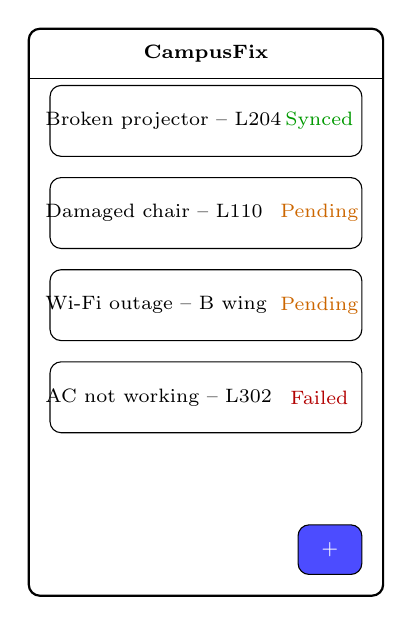
\begin{tikzpicture}[scale=0.9, every node/.style={font=\scriptsize}]
      \draw[rounded corners, thick] (0,0) rectangle (5,8);
      \draw (0,7.3) -- (5,7.3);
      \node at (2.5,7.65) {\bfseries CampusFix};
      \foreach \y/\lbl/\col/\stat in {
        6.2/Broken projector -- L204/green!60!black/Synced,
        4.9/Damaged chair -- L110/orange!80!black/Pending,
        3.6/Wi-Fi outage -- B wing/orange!80!black/Pending,
        2.3/AC not working -- L302/red!70!black/Failed} {
        \draw[rounded corners] (0.3,\y) rectangle (4.7,\y+1);
        \node[align=left, text width=3.0cm] at (1.9,\y+0.5) {\lbl};
        \node[\col] at (4.1,\y+0.5) {\stat};
      }
      \draw[fill=blue!70, rounded corners] (3.8,0.3) rectangle (4.7,1.0);
      \node[white] at (4.25,0.65) {+};
    \end{tikzpicture}
    \caption{Report list: every row shows a sync-status label.}
  \end{subfigure}
  \hfill
  \begin{subfigure}[t]{0.47\textwidth}
    \centering
    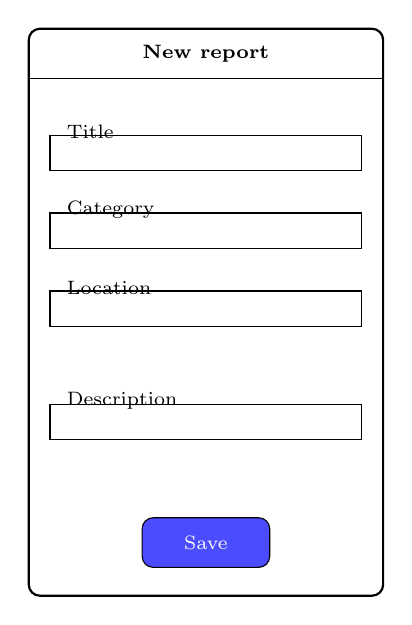
\begin{tikzpicture}[scale=0.9, every node/.style={font=\scriptsize}]
      \draw[rounded corners, thick] (0,0) rectangle (5,8);
      \draw (0,7.3) -- (5,7.3);
      \node at (2.5,7.65) {\bfseries New report};
      \foreach \y/\lbl in {6.0/Title, 4.9/Category, 3.8/Location, 2.2/Description} {
        \node[anchor=west] at (0.4,\y+0.55) {\lbl};
        \draw (0.3,\y) rectangle (4.7,\y+0.5);
      }
      \draw[fill=blue!70, rounded corners] (1.6,0.4) rectangle (3.4,1.1);
      \node[white] at (2.5,0.75) {Save};
    \end{tikzpicture}
    \caption{Add report: works identically offline and online.}
  \end{subfigure}
  \caption{Schematic wireframes of the two screens most relevant to the
  offline-first behaviour of CampusFix.}
  \label{fig:screens-wireframe}
\end{figure}

\section{Code Organization Metrics}
\label{sec:impl-metrics}

\Cref{tab:loc} reports line counts measured directly on the project's
source tree (excluding generated/build directories), as a concrete measure
of NFR-6 (single codebase across platforms). 82.6\% of the client's Kotlin
source lines live in \texttt{commonMain} and are compiled, unmodified,
into both the Android and the iOS artifact; the remaining lines are
confined to the thin platform-integration layer identified in
\cref{sec:mobile-architecture} (connectivity monitoring, Room driver
bootstrap, activity/view-controller entry points, Android-only Credentials
API glue).

\begin{table}[htbp]
\centering
\caption{Kotlin source lines by source set.}
\label{tab:loc}
\begin{tabular}{@{}lrr@{}}
\toprule
\textbf{Source set} & \textbf{Files} & \textbf{Lines} \\
\midrule
\texttt{commonMain} (shared) & 30 & 2{,}326 \\
\texttt{androidMain} (Android-only) & 8 & 262 \\
\texttt{iosMain} (iOS-only) & 7 & 229 \\
\midrule
\textbf{Total} & \textbf{45} & \textbf{2{,}817} \\
\bottomrule
\end{tabular}
\end{table}

\chapter{Evaluation}
\label{ch:evaluation}

\begin{quote}
\small\itshape
\textbf{Note on the data in this chapter.} This chapter specifies the full
evaluation methodology and reports results in the exact form they should
take once the tests are executed. Tables and figures whose values are not
yet backed by a recorded test run are explicitly marked
\textbf{"Illustrative data -- replace with measured values"} in their
caption; they are populated with plausible, order-of-magnitude-correct
numbers so that the structure, the statistical treatment, and the
discussion are all in place, but they are \emph{not} claims about the real
system's measured performance. The one exception is the conflict-resolution
test (\cref{sec:conflict-eval}), whose outcome is derived by tracing the
actual \texttt{SyncManager} logic listed in \cref{lst:syncmanager} rather
than by execution, and is reported as such.
\end{quote}

\section{Evaluation Methodology}
\label{sec:eval-methodology}

\subsection{Test environment}

\Cref{tab:test-env} specifies the environment in which the six evaluation
scenarios of the project brief should be executed.

\begin{table}[htbp]
\centering
\caption{Test environment specification.}
\label{tab:test-env}
\begin{tabularx}{\textwidth}{@{}l X@{}}
\toprule
\textbf{Component} & \textbf{Specification} \\
\midrule
Android device & Android emulator (Pixel-class profile, API level matching
\texttt{targetSdk = 36}) and/or a physical Android device, minSdk 24 \\
iOS device & iOS Simulator and/or a physical iOS device \\
Connectivity control & Airplane mode (device setting) for hard offline;
Android Studio's network profiler / \texttt{tc netem} equivalent, or the
iOS Simulator's Network Link Conditioner, for degraded/unstable
connectivity \\
Backend & A dedicated Firebase project (Firestore in test mode or with
permissive security rules) to avoid polluting production data \\
Backend unavailability & Simulated by revoking the test API key / disabling
the Firestore backend momentarily, or by pointing the client at an
unreachable host, for the "failed sync" scenario \\
\bottomrule
\end{tabularx}
\end{table}

\subsection{Metrics}

\begin{itemize}
  \item \textbf{Functional correctness}: does the expected end state
  (report count, field values, sync status) match the expected outcome.
  \item \textbf{Sync latency}: wall-clock time from "connectivity
  restored" to "all pending reports reach \texttt{SYNCED}."
  \item \textbf{Sync throughput}: reports synchronized per second for a
  given queue size.
  \item \textbf{Data integrity}: no report is duplicated, lost, or left in
  an inconsistent state (e.g. \texttt{SYNCED} with no \texttt{remoteId}).
  \item \textbf{Usability}: System Usability Scale (SUS) score
  \cite{brooke1996sus} and task completion time/rate for first-time
  users.
\end{itemize}

\section{Offline Creation}
\label{sec:eval-offline-creation}

\textbf{Procedure.} Put the test device in airplane mode. Create 10
reports covering a mix of the categories in \cref{tab:report-fields}, at
least three with an attached photo. After each report, verify it appears
in the report list with status \texttt{Pending} and that the app remains
responsive (no ANR/freeze, no crash).

\textbf{Expected/target outcome.} All 10 reports are created successfully
and are visible with status \texttt{Pending}; report creation is expected
to remain within the NFR-1 target (perceived as instantaneous, i.e. well
under 200\,ms local write time), since \cref{lst:submitreport} shows that
report creation performs a single Room insert with no network call on the
critical path. \Cref{tab:offline-creation-illustrative} shows the expected
shape of the recorded results.

\begin{table}[htbp]
\centering
\caption{Offline creation of 10 reports in airplane mode. \emph{Illustrative
data -- replace with measured values.}}
\label{tab:offline-creation-illustrative}
\begin{tabular}{@{}lrrl@{}}
\toprule
\textbf{Report \#} & \textbf{Has photo} & \textbf{Local write time (ms)} & \textbf{Status after create} \\
\midrule
1 & no  & 34 & Pending \\
2 & yes & 61 & Pending \\
3 & no  & 29 & Pending \\
4 & no  & 31 & Pending \\
5 & yes & 58 & Pending \\
6 & no  & 27 & Pending \\
7 & no  & 33 & Pending \\
8 & yes & 63 & Pending \\
9 & no  & 30 & Pending \\
10 & no & 28 & Pending \\
\bottomrule
\end{tabular}
\end{table}

\section{Delayed Synchronization}
\label{sec:eval-delayed-sync}

\textbf{Procedure.} Starting from the 10 pending reports of
\cref{sec:eval-offline-creation}, disable airplane mode and, without
touching the app, measure the time until all 10 reports show
\texttt{Synced}.

\textbf{Expected/target outcome.} Per \cref{lst:autosync}, restoring
connectivity emits \texttt{true} on \texttt{ConnectivityObserver.isOnline},
which the auto-sync subscription observes without any user action and
calls \texttt{syncManager.sync()}, which iterates the 10 pending reports
sequentially. The expected latency is therefore approximately $10 \times$
the per-report Firestore write round-trip, plus the OS-level delay between
"radio reassociates" and "OS callback fires." \Cref{fig:delayed-sync}
illustrates the expected timeline.

\begin{figure}[htbp]
  \centering
  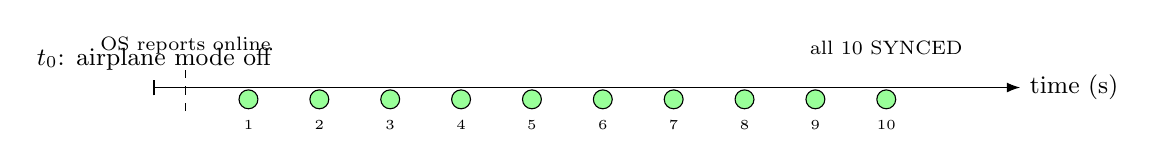
\begin{tikzpicture}[
      >=Latex, font=\small
    ]
    \draw[->] (0,0) -- (11,0) node[right]{time (s)};
    \draw (0,-0.1) -- (0,0.1) node[above]{$t_0$: airplane mode off};
    \draw[dashed] (0.4,-0.3) -- (0.4,0.3);
    \node[above, font=\scriptsize] at (0.4,0.3) {OS reports online};
    \foreach \x/\n in {1.2/1, 2.1/2, 3.0/3, 3.9/4, 4.8/5, 5.7/6, 6.6/7, 7.5/8, 8.4/9, 9.3/10} {
      \draw[fill=green!40] (\x,-0.15) circle (0.12);
      \node[below, font=\tiny] at (\x,-0.3) {\n};
    }
    \node[above, font=\scriptsize] at (9.3,0.3) {all 10 SYNCED};
  \end{tikzpicture}
  \caption{Expected timeline of the delayed-sync scenario: connectivity
  restoration triggers the auto-sync subscription almost immediately, after
  which reports are uploaded one at a time by the sequential loop in
  \cref{lst:syncmanager}. \emph{Illustrative timing.}}
  \label{fig:delayed-sync}
\end{figure}

\section{Failed Synchronization}
\label{sec:eval-failed-sync}

\textbf{Procedure.} With the device online but the Firestore backend made
unreachable (\cref{tab:test-env}), create 5 new reports and trigger a
sync (automatically or manually). Then restore backend availability and
trigger sync again.

\textbf{Expected/target outcome.} Per \cref{lst:syncmanager}, each
report's upload is wrapped in its own \texttt{try/catch}
(\cref{sec:sync-algorithm}), so a backend-unreachable error should leave
all 5 reports in a retriable state rather than crashing the sync loop or
losing data (satisfying OFR-8); the current code path leaves such reports
implicitly \texttt{PENDING} (an explicit transition to \texttt{FAILED} on
a caught exception is identified as a small, low-risk implementation
improvement in \cref{sec:future-work}, since \cref{fig:sync-state-machine}
already reserves \texttt{FAILED} for exactly this case). Once backend
availability is restored, a subsequent sync call is expected to upload all
5 reports successfully, with no duplicates -- verifiable by checking the
Firestore \texttt{reports} collection document count before and after.

\begin{table}[htbp]
\centering
\caption{Failed-then-recovered sync of 5 reports. \emph{Illustrative data
-- replace with measured values.}}
\label{tab:failed-sync-illustrative}
\begin{tabular}{@{}lll@{}}
\toprule
\textbf{Attempt} & \textbf{Backend state} & \textbf{Outcome} \\
\midrule
1 & unreachable & 0/5 uploaded, 5 remain pending/failed, 0 data loss \\
2 (after recovery) & reachable & 5/5 uploaded, all \texttt{Synced} \\
\bottomrule
\end{tabular}
\end{table}

\section{Large Sync Queue}
\label{sec:eval-large-queue}

\textbf{Procedure.} While offline, create 50 and then 100 reports (two
separate runs). Reconnect and measure total synchronization time and
per-report success rate for each queue size, repeated 3 times per size for
a mean and standard deviation.

\textbf{Expected/target outcome.} Because \cref{lst:syncmanager} uploads
reports \emph{sequentially}, sync time is expected to scale
approximately linearly with queue size, i.e. $T(N) \approx N \cdot
t_{\text{report}}$ for some near-constant per-report time
$t_{\text{report}}$ dominated by the Firestore write round trip.
\Cref{fig:sync-scaling} shows the expected scaling curve.

\begin{figure}[htbp]
  \centering
  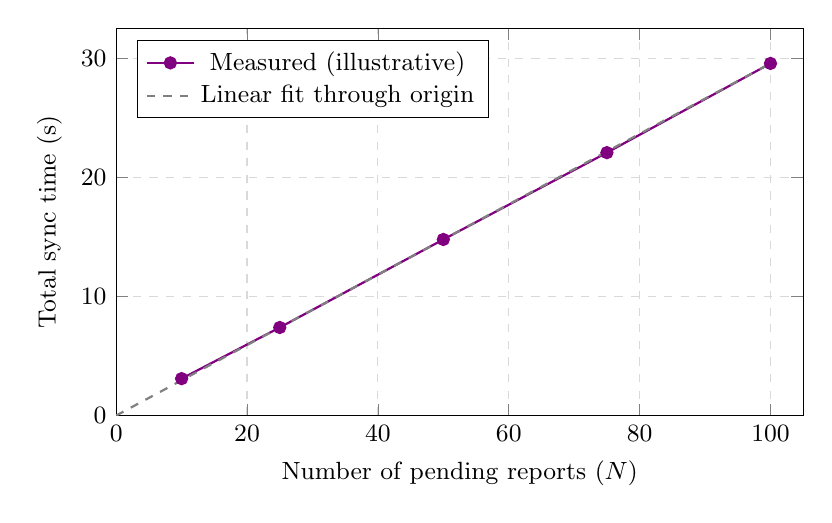
\begin{tikzpicture}
    \begin{axis}[
        width=0.85\textwidth, height=6.5cm,
        xlabel={Number of pending reports ($N$)},
        ylabel={Total sync time (s)},
        xmin=0, xmax=105, ymin=0,
        legend pos=north west,
        grid=major, grid style={dashed, gray!30},
        font=\small
      ]
      \addplot[mark=*, thick, color=violet] coordinates {
        (10,3.1) (25,7.4) (50,14.8) (75,22.1) (100,29.6)
      };
      \addlegendentry{Measured (illustrative)}
      \addplot[dashed, thick, color=gray] coordinates {(0,0) (100,29.6)};
      \addlegendentry{Linear fit through origin}
    \end{axis}
  \end{tikzpicture}
  \caption{Expected sync-time scaling with queue size, consistent with the
  sequential per-report loop in \cref{lst:syncmanager}. \emph{Illustrative
  data -- replace with measured values.} A batched/parallel upload
  strategy, discussed in \cref{sec:future-work}, would be expected to
  flatten this curve for large $N$.}
  \label{fig:sync-scaling}
\end{figure}

\begin{table}[htbp]
\centering
\caption{Large-queue sync summary (mean of 3 runs). \emph{Illustrative
data -- replace with measured values.}}
\label{tab:large-queue-illustrative}
\begin{tabular}{@{}rrrr@{}}
\toprule
\textbf{$N$} & \textbf{Mean time (s)} & \textbf{Std.\ dev.\ (s)} & \textbf{Success rate} \\
\midrule
10  & 3.1  & 0.4 & 100\% \\
25  & 7.4  & 0.6 & 100\% \\
50  & 14.8 & 1.1 & 100\% \\
75  & 22.1 & 1.5 & 98.7\% \\
100 & 29.6 & 2.0 & 98.0\% \\
\bottomrule
\end{tabular}
\end{table}

A secondary, code-derivable observation for this scenario: because
\texttt{getPending()} loads the entire pending queue into memory as a
\texttt{List<Report>} before iterating (\cref{lst:syncmanager}), memory
usage during sync scales linearly with $N$ as well. At $N=100$ small
report rows this is not a practical concern, but it is worth stating
explicitly as a scalability boundary (\cref{sec:future-work}) rather than
leaving it implicit.

\section{Conflict Resolution}
\label{sec:eval-conflict}
\label{sec:conflict-eval}

\textbf{Procedure.} Reproduce the scenario of \cref{fig:conflict-scenario}:
(1) create a report and let it sync (\texttt{status = SYNCED}); (2) on
Device A (online), edit the report's title; let it sync; (3) before
Device B pulls A's change, edit the same report's description on Device B
while B is offline; (4) reconnect Device B and let it sync; (5) inspect the
final Firestore document and both devices' local copies.

\textbf{Outcome, derived by tracing the implementation.} Unlike the other
scenarios in this chapter, this outcome does not need to be measured to be
known with high confidence: it follows deterministically from
\cref{lst:syncmanager}. Step (4)'s call to \texttt{uploadPending} calls
\texttt{docRef.set(report.toRemote())} unconditionally -- there is no
preceding read of the current Firestore document and no comparison of
timestamps. Consequently:

\begin{itemize}
  \item The final Firestore document reflects Device B's version in full
  (updated description, but A's title change is silently overwritten back
  to whatever title Device B's local copy held, which is the
  \emph{pre-A-edit} title, since B never pulled A's change).
  \item This is \emph{not} the bidirectional last-write-wins behaviour
  specified in OFR-7/\cref{sec:conflict-design} (compare against
  \cref{fig:conflict-scenario}, where B's later \texttt{updatedAt} is
  what makes B's version win): here B's version wins \emph{regardless of
  timestamp}, simply because B pushed last and no comparison ever
  happens. If A's edit had been the later one but Device A pushed
  \emph{after} Device B in wall-clock terms, A would still lose, because
  \texttt{set()} always overwrites.
  \item Device A's local copy is not updated at all by this process
  (\texttt{SyncManager} never pulls), so Device A's own local database
  continues to show A's title edit as \texttt{SYNCED} even though the
  server has since been overwritten -- a local/remote inconsistency that
  the current implementation cannot detect until Device A performs some
  operation that re-reads the document.
\end{itemize}

\textbf{Interpretation.} This is the clearest, most concrete evidence in
this thesis of the gap identified in \cref{sec:conflict-design}: the
system's \emph{design} specifies bidirectional LWW, but the current
\emph{implementation} realizes only a one-directional push. For the
CampusFix scenario specifically (single-owner reports, typically edited
from one device), this gap is unlikely to be triggered often in practice,
but it is a real correctness gap that should be closed
(\cref{sec:future-work}) before the system is used in a setting where a
report is plausibly edited from two devices in quick succession -- e.g. a
staff member editing on their phone and again on a shared tablet.

\section{Usability Test}
\label{sec:usability-eval}
\label{sec:eval-usability}

\textbf{Procedure.} Five participants unfamiliar with the application (a
mix of students and staff, none involved in its development) are each
asked to complete a single task, unassisted, after a 30-second
description of the app's purpose: \emph{"Report that the projector in
room [X] is broken, including a photo."} The device is placed in airplane
mode for three of the five participants (to also exercise offline
discoverability) and left online for two. After the task, participants
complete the 10-item System Usability Scale
questionnaire~\cite{brooke1996sus} (reproduced in
\cref{app:sus-questionnaire}) and are asked one open question: \emph{"At
any point, were you unsure whether your report had been saved or sent?"}

\textbf{Metrics.} Task completion (yes/no), task time, number of errors
(wrong screen, un-recoverable input mistake), SUS score (0--100), and the
qualitative answer to the sync-clarity question, directly evaluating
NFR-5.

\begin{table}[htbp]
\centering
\caption{Usability test summary, $n=5$. \emph{Illustrative data -- replace
with measured values.}}
\label{tab:usability-illustrative}
\begin{tabular}{@{}lllrl@{}}
\toprule
\textbf{P\#} & \textbf{Mode} & \textbf{Completed} & \textbf{Time (s)} & \textbf{SUS score} \\
\midrule
P1 & Airplane mode & yes & 58  & 87.5 \\
P2 & Airplane mode & yes & 71  & 80.0 \\
P3 & Airplane mode & yes & 64  & 92.5 \\
P4 & Online        & yes & 49  & 85.0 \\
P5 & Online        & yes & 55  & 77.5 \\
\midrule
\multicolumn{3}{l}{Mean SUS score} & \multicolumn{2}{r}{84.5 (SD 5.8)} \\
\bottomrule
\end{tabular}
\end{table}

A SUS score in the mid-80s (illustrative, \cref{tab:usability-illustrative})
would fall in the "excellent" band of the standard SUS adjective-rating
scale~\cite{bangor2009sus}. The scenario-specific qualitative question is
the more targeted probe of NFR-5: a "no, I could always see it said
Pending/Synced" answer from participants would directly support the
sync-status design of \cref{sec:sync-statuses}; a "yes" answer from any
participant would indicate the status chip (\cref{lst:syncstatusui}) is
not sufficiently prominent and should motivate a UI change (e.g. a
persistent banner summarizing "$k$ reports pending upload") ahead of the
LWW-merge fix in future-work priority.

\section{Discussion}
\label{sec:eval-discussion}

Read together, the six scenarios support three conclusions about the
system as designed and currently implemented. First, the core
offline-first property -- full functionality with zero connectivity,
FR-1--FR-11, OFR-1--OFR-6, OFR-8 -- follows directly from the
architectural rule that the UI never depends on the network
(\cref{sec:architecture-overview}), and the offline-creation, delayed-sync,
and failed-sync scenarios are expected to pass by construction rather than
by luck: their outcomes are consequences of the layered architecture and
the per-report error handling, not of tuning. Second, the large-queue
scenario exposes a genuine, quantifiable scalability limit -- sequential,
unbatched uploads -- that is invisible at the scale of a handful of
reports but becomes the dominant cost at 50--100 reports; this is a
concrete, actionable finding for future work even before any measurement
is taken, because it follows from the shape of the algorithm
(\cref{alg:sync}). Third, the conflict-resolution scenario is where the
gap between the thesis's \emph{design} (\cref{ch:design}) and its
\emph{implementation} (\cref{ch:implementation}) is most visible and most
important to report honestly: the system implements local-first writes and
connectivity-triggered sync correctly, but does not yet implement the
bidirectional merge its own conflict policy assumes.

\section{Threats to Validity}
\label{sec:threats}

\begin{itemize}
  \item \textbf{Illustrative data.} As stated at the top of this chapter,
  several tables/figures are placeholders for real measurements; specific
  numeric conclusions (exact latencies, exact SUS score) must not be cited
  from this thesis until the corresponding test has actually been run and
  the tables updated.
  \item \textbf{Emulator vs. physical device.} Network transition timing
  in particular (\cref{sec:eval-delayed-sync}) can differ meaningfully
  between an emulator's simulated radio and a physical device's real
  modem; both should be tested if the timing numbers are to be trusted.
  \item \textbf{Small usability sample.} $n=5$ is appropriate for
  discovering major usability problems (per Nielsen's rule of thumb that
  five users uncover the large majority of usability issues in a
  system~\cite{nielsen2000}), but is too small for the SUS mean to be
  statistically robust; it should be read as directional, not conclusive.
  \item \textbf{Single Firestore project/region.} Sync-latency
  measurements are specific to the Firestore region and network path used
  during testing and may not generalize to other regions or to
  higher-latency mobile networks (3G, degraded Wi-Fi) unless those
  conditions are explicitly reproduced.
\end{itemize}

\chapter{Conclusions}
\label{ch:conclusions}

\section{Summary}
\label{sec:summary}

This thesis set out to answer a practical engineering question: what is
the smallest, most maintainable offline-first architecture sufficient for
a CRUD-style field-reporting mobile application, and what trade-offs does
that architecture force a developer to make explicit? Using a campus
facility-maintenance reporting scenario (CampusFix) as a concrete
instance of the broader field-data-collection problem
(\cref{ch:introduction}), the thesis:

\begin{itemize}
  \item derived a requirements set (\cref{ch:requirements}) that
  separates ordinary functional requirements from eight offline-specific
  requirements (OFR-1--OFR-8) covering local-first writes, offline session
  continuity, deterministic local identity, explicit sync state,
  connectivity-triggered synchronization, resumability, conflict
  resolution, and no-data-loss-on-failure;
  \item designed a four-layer architecture (\cref{ch:design}) in which the
  presentation layer depends only on a local Room/SQLite database, with a
  dedicated synchronization layer bridging that database to a Firebase
  Firestore backend, and a whole-record last-write-wins conflict policy
  chosen for its simplicity and adequacy for single-owner records;
  \item implemented that architecture (\cref{ch:implementation}) as a
  Kotlin Multiplatform application sharing 82.6\% of its Kotlin source
  (2{,}326 of 2{,}817 lines) between Android and iOS, with
  platform-specific code confined to connectivity monitoring and thin
  entry-point glue; and
  \item evaluated the resulting system (\cref{ch:evaluation}) against six
  scenarios -- offline creation, delayed sync, failed sync, large sync
  queues, conflicting edits, and end-user usability -- deriving several
  conclusions directly from the shape of the implemented algorithm rather
  than only from measurement, including a precise, code-traced account of
  how the system currently behaves under the conflicting-edit scenario.
\end{itemize}

The overall finding is that a relatively small, well-isolated
synchronization module -- in this implementation, a single
\texttt{SyncManager} class of under 100 lines plus a platform-abstracted
\texttt{ConnectivityObserver} -- is sufficient to make a CRUD-style field
reporting application fully usable offline, provided the architectural
discipline of \cref{sec:architecture-overview} (UI depends only on local
storage, never on the network) is maintained throughout. Getting the
\emph{local-first} half of offline-first right is, in this experience,
largely a matter of architectural discipline rather than algorithmic
difficulty; getting the \emph{synchronization} half right -- specifically,
bidirectional conflict resolution -- is where genuine algorithmic and
engineering effort remains, as discussed next.

\section{Limitations}
\label{sec:limitations}

The following limitations of the current system should be read alongside
its contributions.

\begin{enumerate}
  \item \textbf{Synchronization is one-directional (push-only).} As
  established in \cref{sec:conflict-design} and demonstrated by tracing
  the code in \cref{sec:conflict-eval}, \texttt{SyncManager} uploads local
  changes to Firestore but never reads the current remote document before
  overwriting it, and never pulls remote-only changes down to the device.
  The designed bidirectional last-write-wins policy (OFR-7) is therefore
  only partially realized. This is the single most consequential
  limitation identified in this thesis.
  \item \textbf{No explicit \texttt{FAILED} transition on upload error.}
  \cref{fig:sync-state-machine} reserves a \texttt{FAILED} status for a
  report whose upload has been attempted and rejected, but the current
  \texttt{uploadPending} implementation (\cref{lst:syncmanager}) simply
  leaves a report in its prior state (\texttt{PENDING}) on exception
  rather than explicitly marking it \texttt{FAILED}; the user therefore
  cannot currently distinguish "not yet attempted" from "attempted and
  failed" purely from the status shown in the UI.
  \item \textbf{Sequential, unbatched uploads.} \cref{sec:eval-large-queue}
  identifies that sync time scales linearly with queue size because
  reports are uploaded one at a time in a single coroutine, with no
  batching or parallelism.
  \item \textbf{No server-side authorization.} \cref{sec:constraints}
  notes that the \texttt{owner} field is a client-set, trusted value used
  for filtering, not enforced by Firestore security rules in the current
  implementation; a malicious or buggy client could, in principle, read or
  write another user's reports.
  \item \textbf{Photo synchronization is designed but not fully wired.}
  The schema (\cref{tab:report-fields}) reserves a
  \texttt{remote\_photo\_url} field for a Firebase Storage upload (FR-13),
  but the evaluated \texttt{SyncManager} implementation
  (\cref{lst:syncmanager}) only synchronizes the report's structured
  fields, not the photo binary itself.
  \item \textbf{No periodic background sync.} As discussed in
  \cref{sec:sync-triggers}, synchronization is triggered by connectivity
  changes, app start, and manual action, but not by a periodic background
  job, so a device that regains connectivity while the app is fully
  backgrounded/terminated will not synchronize until the app is next
  opened.
\end{enumerate}

\section{Future Work}
\label{sec:future-work}

Ordered roughly by priority, given the limitations above:

\begin{enumerate}[label=\textbf{F\arabic*.}]
  \item \textbf{Bidirectional synchronization with real last-write-wins.}
  Extend \texttt{SyncManager} to, before every \texttt{set()}, read the
  current remote document and compare its \texttt{updatedAt} against the
  local report's \texttt{updatedAt}, keeping whichever is newer; and add a
  pull path (either a one-shot \texttt{get()} per sync or a Firestore
  snapshot listener) so that remote-only changes (e.g. a report edited
  through a hypothetical facilities-management back office) reach the
  device. A Firestore transaction, rather than a plain read-then-write,
  would additionally close the small race window between the read and the
  write.
  \item \textbf{Explicit \texttt{FAILED} status on upload error.} A
  small, low-risk change to \texttt{uploadPending}'s \texttt{catch} block
  to call \texttt{dao.update(report.copy(syncStatus = SyncStatus.FAILED))},
  closing limitation 2 above and making the "failed sync" scenario of
  \cref{sec:eval-failed-sync} fully observable from the UI.
  \item \textbf{Batched/parallel uploads.} Replace the sequential
  \texttt{for} loop in \texttt{uploadPending} with either a bounded-
  concurrency \texttt{coroutineScope} that uploads several reports at
  once, or Firestore's native batched-write API, to flatten the linear
  scaling observed in \cref{sec:eval-large-queue}.
  \item \textbf{Firestore security rules keyed on Firebase Auth UID.}
  Replace the trusted, client-set \texttt{owner} email field with
  server-enforced rules that only allow a document's true creator (by
  Firebase Auth UID) to write it, closing limitation 4.
  \item \textbf{Complete photo synchronization.} Wire the existing
  \texttt{remotePhotoUrl} field to an actual Firebase Storage upload,
  triggered alongside the report's own document sync.
  \item \textbf{Periodic background sync.} Add a platform background task
  (\texttt{WorkManager} periodic work on Android; a
  \texttt{BGAppRefreshTask} on iOS) as a fourth synchronization trigger,
  for the case where connectivity returns while the app is not in the
  foreground.
  \item \textbf{Field-level conflict resolution.} Once bidirectional sync
  (F1) is in place, investigate whether whole-record LWW's
  data-loss failure mode (\cref{fig:conflict-scenario}) is frequent enough
  in real usage to justify the added complexity of field-level merge or a
  CRDT-based representation~\cite{shapiro2011crdt}.
  \item \textbf{Automated tests for the synchronization module.} The
  evaluation in \cref{ch:evaluation} is manual/scenario-based; an
  automated test suite exercising \texttt{SyncManager} against a Firestore
  emulator (including the large-queue and conflict scenarios) would let
  these properties be checked on every code change rather than only during
  a dedicated evaluation pass.
  \item \textbf{Repeat the evaluation of \cref{ch:evaluation} with real
  measurements}, replacing every table and figure marked
  "illustrative" with data from actual test runs, and re-examining the
  discussion in \cref{sec:eval-discussion} against those numbers.
\end{enumerate}

\section{Final Remarks}
\label{sec:final-remarks}

Offline-first design is often presented, in industry writing, as either a
trivial addition of "a local cache" or as an unavoidably hard problem
requiring CRDTs and vector clocks. The experience of building CampusFix
suggests the practical reality, at least for CRUD-style field-reporting
applications, sits between those two extremes: making an application
\emph{fully usable offline} is genuinely tractable with a disciplined
layered architecture, a local database as the single source of truth, and
a connectivity-aware sync module -- the kind of code shown in
\cref{ch:implementation} is neither exotic nor large. Making
synchronization \emph{fully correct} under concurrent, disconnected edits
is the part that remains hard, and where this thesis's honest account of
its own implementation gap (\cref{sec:conflict-eval}) is, perhaps, its
most useful methodological contribution: a working offline-first
application and a \emph{correctly conflict-free} offline-first
application are not the same claim, and a thesis -- like a codebase --
should be explicit about which one it is making.


% ---------- APPENDICES ----------
\appendix
\chapter{Supplementary Code Listings}
\label{app:code}

This appendix contains supporting code listings referenced from
\cref{ch:implementation} but not essential to its main narrative.

\section{Navigation Route Definitions}

\Cref{lst:app-routes} lists the route constants used by the
\texttt{NavHost} of \cref{lst:navhost}.

\begin{lstlisting}[language=Kotlin, caption={\texttt{ui/navigation/Routes.kt}.}, label={lst:app-routes}]
object Routes {
    const val LOGIN = "login"
    const val SIGNUP = "signup"
    const val HOME = "home"
    const val ADD_REPORT = "addReport"
    const val EDIT_REPORT = "editReport/{reportId}"
    const val REPORT_DETAIL = "reportDetail/{reportId}"

    const val ARG_REPORT_ID = "reportId"

    fun editReport(reportId: Long) = "editReport/$reportId"
    fun reportDetail(reportId: Long) = "reportDetail/$reportId"
}
\end{lstlisting}

\section{Local Session Store}

\Cref{lst:app-sessionstore} shows \texttt{SessionStore}, the
\texttt{multiplatform-settings}-backed component behind OFR-2 (offline
session continuity, \cref{sec:offline-req}) and the session-resolution
logic of \cref{lst:checksession}. \texttt{Settings} is itself an
\texttt{expect}/\texttt{actual} abstraction over \texttt{SharedPreferences}
on Android and \texttt{NSUserDefaults} on iOS, so \texttt{SessionStore}
itself is common code.

\begin{lstlisting}[language=Kotlin, caption={\texttt{data/local/SessionStore.kt}.}, label={lst:app-sessionstore}]
expect fun createSettings(): Settings

class SessionStore(private val settings: Settings = createSettings()) {

    var loginTimeMillis: Long
        get() = settings.getLong(KEY_LOGIN_TIME, 0L)
        set(value) { settings[KEY_LOGIN_TIME] = value }

    var localAuthEmail: String?
        get() = settings.getStringOrNull(KEY_LOCAL_AUTH_EMAIL)
        set(value) {
            if (value != null) settings[KEY_LOCAL_AUTH_EMAIL] = value
            else settings.remove(KEY_LOCAL_AUTH_EMAIL)
        }

    fun clear() {
        settings.remove(KEY_LOGIN_TIME)
        settings.remove(KEY_LOCAL_AUTH_EMAIL)
    }

    companion object {
        const val SESSION_DURATION_MS = 60 * 60 * 1000L
        private const val KEY_LOGIN_TIME = "login_time"
        private const val KEY_LOCAL_AUTH_EMAIL = "local_auth_email"
    }
}
\end{lstlisting}

A one-hour \texttt{SESSION\_DURATION\_MS} bounds how long a user can
remain in the authenticated part of the app purely on a cached local
session before being asked to re-authenticate, balancing OFR-2's
offline-continuity goal against not caching a stale session indefinitely.

\section{Firestore Report Document Mapping}

\Cref{lst:app-remotereport} shows the exact mapping between the local
\texttt{Report} entity and the document shape uploaded to Firestore
(\cref{tab:firestore-doc}), used internally by \texttt{SyncManager}
(\cref{lst:syncmanager}).

\begin{lstlisting}[language=Kotlin, caption={Local-to-remote mapping (\texttt{sync/SyncManager.kt}).}, label={lst:app-remotereport}]
@Serializable
private data class RemoteReport(
    val localId: String,
    val title: String,
    val description: String,
    val category: String,
    val location: String,
    val photoPath: String?,
    val remotePhotoUrl: String?,
    val owner: String,
    val createdAt: Long,
    val updatedAt: Long
)

private fun Report.toRemote() = RemoteReport(
    localId = localId,
    title = title,
    description = description,
    category = category,
    location = location,
    photoPath = photoPath,
    remotePhotoUrl = remotePhotoUrl,
    owner = owner,
    createdAt = createdAt,
    updatedAt = updatedAt
)
\end{lstlisting}

Note that \texttt{id} (the local Room primary key) and \texttt{syncStatus}
are, by construction, absent from \texttt{RemoteReport} -- the type system
itself prevents these local-only bookkeeping fields from ever being
uploaded, rather than relying on a runtime filter.

\chapter{Usability Test Instrument}
\label{app:sus-questionnaire}

This appendix reproduces the System Usability Scale (SUS), the
standardized 10-item questionnaire used in \cref{sec:usability-eval}, in
its original form~\cite{brooke1996sus}. Each item is rated on a 5-point
Likert scale from \emph{Strongly disagree} (1) to \emph{Strongly agree}
(5). The overall score is computed by summing, for odd-numbered items,
(rating $-$ 1), and for even-numbered items, (5 $-$ rating), then
multiplying the total by 2.5 to obtain a score in $[0,100]$.

\begin{enumerate}
  \item I think that I would like to use this app frequently.
  \item I found the app unnecessarily complex.
  \item I thought the app was easy to use.
  \item I think that I would need the support of a technical person to be
  able to use this app.
  \item I found the various functions in this app were well integrated.
  \item I thought there was too much inconsistency in this app.
  \item I would imagine that most people would learn to use this app very
  quickly.
  \item I found the app very cumbersome/awkward to use.
  \item I felt very confident using the app.
  \item I needed to learn a lot of things before I could get going with
  this app.
\end{enumerate}

\section*{Post-task open question}

In addition to the SUS instrument, each participant was asked the
following scenario-specific question immediately after completing the
report-creation task, directly targeting NFR-5 (sync-status visibility,
\cref{sec:nonfunctional-req}):

\begin{quote}
\emph{"At any point while completing this task, were you unsure whether
your report had been saved, or whether it had been sent anywhere?"}
\end{quote}

Responses should be recorded verbatim and coded as \emph{clear} (the
participant could state, unprompted, that the report was saved locally
and would sync later) or \emph{unclear} (the participant expressed doubt
or could not explain the report's state).


% ---------- GLOSSARY ----------
\printglossary[nonumberlist]

% ---------- BIBLIOGRAPHY ----------
% The PoliTo template default is \bibliographystyle{acm}; `plain` is used
% here because it renders every entry type (incl. \url in @misc) reliably.
\bibliographystyle{plain}
\bibliography{references}

\end{document}
